\documentclass[dvipsnames, svgnames, x11names]{beamer}
\usetheme{mytheme2024}
% \special{dvipdfmx:config z 0} %取消PDF压缩，加快速度，最终版本生成的时候最好把这句话注释掉

\title{化学反应工程}
\subtitle{反应动力学基础}
\author{张斌}
\institute[理工系]{河北农业大学 理工系}
\date{\the\year 年 \the\month 月}
%-----------------------------------------------------------------
\begin{document}

\maketitle


\begin{frame}
	\frametitle{本章研究内容}
	\qquad \Large 反应动力学是研究化学反应速率以及各种因素对反应速率影响的学科。传统上属于物理化学的范围，但为了满足工程实践的需要，化学反应工程在其发展过程中，在这方面也进行了大量的研究工作。本章将在物理化学基础上，从反应工程学科的角度阐明某些常用的反应动力学概念和动力学问题的处理方法，包括\bf{均相反应动力学}及\bf{多相催化反应动力学}。
\end{frame}


\begin{frame}{}
	\begin{center}
		\Huge \cbf{目 \ 录}
	\end{center}
	\tableofcontents
\end{frame}





\section{化学计量学}


% \begin{frame}
%     \frametitle{化学计量方程}
%     化学反应方程式：描述反应物和产物的化学反应过程的定量关系式
%     \[
%         \ch{aA + bB -> cC + dD}
%     \]

%     化学计量方程：只表示反应物和产物在化学反应过程中量的变化关系。
%     \[
%         {\nu_\mathrm{A}\mathrm{A}}+{\nu_\mathrm{B}\mathrm{B}}\to{\nu_\mathrm{C}\mathrm{C}}+ {\nu_\mathrm{D}\mathrm{D}}
%     \]
% \end{frame}


\begin{frame}
    \frametitle{化学反应进行的程度}
    \begin{question}
      合成氨反应：
      \begin{center}
          \ch{N2 + 3 H2 -> 2 NH3}
  
      反应开始(mol)： \qquad 3  \quad   10 \qquad  \qquad 0 \qquad  \qquad \qquad  \qquad  \qquad  \qquad
  
      反应结束(mol)： \qquad  1  \quad ~  4  \qquad  \qquad 4 \qquad \qquad \qquad  \qquad  \qquad  \qquad  \qquad
      \end{center}
      
      这个反应进行了多少？
    \end{question}
\end{frame}


\begin{frame}
    \frametitle{反应进度($\xi$)}
    \[
        {\nu_\mathrm{A}}{A}+{\nu_\mathrm{B}}{B}\to{\nu_\mathrm{R}}{R}
    \]
    \[
        (n_{\mathrm{A}}-n_{\mathrm{A0}}):(n_{\mathrm{B}}-n_{\mathrm{B0}}):(n_{\mathrm{R}}-n_{\mathrm{R0}})=\nu_{\mathrm{A}}:\nu_{\mathrm{B}}:\nu_{\mathrm{R}}
    \]
    \[
        \frac{n_{\mathrm{A}}-n_\mathrm{A0}}{\nu_{\mathrm{A}}}=\frac{n_{\mathrm{B}}-n_\mathrm{B0}}{\nu_{\mathrm{B}}}=\frac{n_{\mathrm{R}}-n_\mathrm{R0}}{\nu_{\mathrm{R}}}=\xi 
    \]
    任何反应组分的反应量与其化学计量系数的之比恒为定值。这里的$\xi$ 叫做反应进度，量纲为mol。可见，只用一个变量便可描述一个化学反应进行的程度。

    推广到任何反应，表示为：
    \[
        \xi=\frac{n_\mathrm{i}-n_\mathrm{i0}}{\nu_\mathrm{i}}
    \]
    \begin{itemize}
      \item $\xi$永远取正值
    \end{itemize}
\end{frame}


\begin{frame}[t]
    \frametitle{反应进度$\xi$的值与方程式的写法有关}
    \begin{block}{反应进度$\xi$为多少？}
        \begin{center}
            \ch{N2 + 3 H2 -> 2 NH3}
    
        反应开始(mol)： \qquad 3  \quad   10 \qquad  \qquad 0 \qquad  \qquad \qquad  \qquad  \qquad  \qquad
    
        反应结束(mol)： \qquad  1  \quad ~  4  \qquad  \qquad 4 \qquad \qquad \qquad  \qquad  \qquad  \qquad  \qquad
        \end{center}
    \end{block}
    \begin{block}{反应进度$\xi$为多少？}
        \begin{center}
            \ch{1/2 N2 + 3/2 H2 -> NH3}
    
        反应开始(mol)： \qquad 3  \qquad   10 \quad  \qquad 0 \qquad  \qquad \qquad  \qquad  \qquad  \qquad
    
        反应结束(mol)： \qquad  1  \qquad ~  4  \quad  \qquad 4 \qquad \qquad \qquad  \qquad  \qquad  \qquad  \qquad
        \end{center}
    \end{block}
\end{frame}


\begin{frame}
    \frametitle{转化率($X$)}
    普遍使用转化率来表示一个化学反应进行的程度。

    转化率是指某一反应物转化的百分率或分率，用$X$表示。
    \[
      X = \frac{\text{某一反应物的转化量}}{\text{该反应物的起始量}}
    \]
    \smallskip
    \[
        X = \frac{n_\mathrm{i0}-n_\mathrm{i}}{n_\mathrm{i0}}
    \]
    \begin{enumerate}
      \item 转化率是针对反应物而言的
      \item 根据不同反应物计算得到的转化率数值可能是不一样的
      \item 工业反应过程的原料中，各反应组分之间往往不符合化学计量数的关系，此时通常选择不过量的反应物计算转化率，这样的组分称为关键组分。
    \end{enumerate}

\end{frame}


\begin{frame}[t]
    \frametitle{}
    \begin{example}
        合成聚氯乙烯单体的合成反应如下：\ch{C2H2 + HCl -> CH2=CHCl}。由于乙炔价格高于氯化氢，通常使用的原料混合气中氯化氢是过量的，设其过量10\%。若反应器出口气体中氯乙烯含量摩尔分数为90\%，分别计算乙炔和氯化氢的转化率。
    \end{example}
    \pause
    \begin{figure}[htpb]
        \centering
        
\includegraphics[width=.65\linewidth]{答案}
    \end{figure}
\end{frame}


\begin{frame}
    \frametitle{转化率起始状态的选择}
    \begin{itemize}
      \item 连续反应器：以反应器进口原料的状态作为起始状态；
      \item 间歇反应器：以反应开始时的状态为起始状态；
      \item 当数个反应器串联时，往往以进入第一个反应器的原料组成作为起始状态。
    \end{itemize}
    \begin{figure}[htpb]
      \centering
      
\includegraphics[width=.8\linewidth]{串联}
    \end{figure}
\end{frame}


\begin{frame}
    \frametitle{收率($Y$)}
    \[
        {\nu_\mathrm{A}}{A}+{\nu_\mathrm{B}}{B}\to{\nu_\mathrm{R}}{R}+{\nu_\mathrm{P}}{P}
    \]

    转化率系针对反应物而言，收率则是针对反应产物而言，其定义为
    \[
        Y_\mathrm{R}=\left|\frac{\nu_\mathrm{A}}{\nu_\mathrm{R}}\right|\frac{\text{反应产物的生成量}}{\text{关键组分的起始量}}
    \]
    \[
        Y=\frac{\text{生成反应产物所消耗的关键组分量}}{\text{关键组分的起始量}}
    \]
    \begin{itemize}
      \item 收率可表明目的产物的相对生成量
      \item 对于单一反应，收率与按关键组分计算的转化率数值上相等，且无论按哪一个反应产物计算的收率数值上都相等。
    \end{itemize}
\end{frame}


\begin{frame}[t]
    \frametitle{}
    \begin{block}{例1.1}
      合成聚氯乙烯单体的合成反应如下：\ch{C2H2 + HCl -> CH2=CHCl}

      由于乙炔价格高于氯化氢，通常使用的原料混合气中氯化氢是过量的，设其过量10\%。若反应器出口气体中氯乙烯含量摩尔分数为90\%，计算聚氯乙烯单体的收率。
    \end{block}
\end{frame}


\begin{frame}[t]
    \frametitle{复合反应的收率}
    \begin{example}
        在银催化剂上进行乙烯氧化反应：

        \ch{C2H4 + 1/2 O2 -> CH2CH2O}

        \ch{C2H4 + 3 O2 -> 2 CO2 + 2 H2O}
        
        进入的乙烯量为100mol，反应器出口环氧乙烷20mol，二氧化碳30mol。求乙烯的转化率，环氧乙烷的收率和\ch{CO2}的收率。
    \end{example}
\end{frame}


\begin{frame}
    \frametitle{反应选择性($S$)}
    一个反应变量只能描述一个反应的进行程度，若多个反应，则反应变量要相应增多。
    \begin{center}
      \ch{C2H4 + 1/2 O2 -> CH2CH2O}

      \ch{C2H4 + 3 O2 -> 2 CO2 + 2 H2O}
    \end{center}
    如果只知道乙烯的转化率，它只说明两个反应的总结果，而不能说明有多少转化成环氧乙烷，又有多少转化成二氧化碳。所以需要再增加一个反应变量，才能对该反应系统作完整描述。
    
    评价复合反应时，除采用转化率和收率外，还可用反应\highlight{选择性}这一概念：
    \[
        S = \frac{\text{生成目的产物所消耗的关键组分量}}{\text{已转化的关键组分量}}
    \]
\end{frame}


\begin{frame}
    \frametitle{转化率、收率、选择性的关系}
    \[
      X = \frac{\text{某一反应物的转化量}}{\text{该反应物的起始量}}
    \]
    \[
        Y=\frac{\text{生成反应产物所消耗的关键组分量}}{\text{关键组分的起始量}}
    \]
    \[
        S = \frac{\text{生成目的产物所消耗的关键组分量}}{\text{已转化的关键组分量}}
    \]
    转化率、收率、选择性的关系：
    \[
        Y = SX
    \]
\end{frame}


\begin{frame}[t]
    \frametitle{}
    \begin{example}
      乙烷脱氢生产乙烯时， 原料乙烷处理量为8000kg/h，产物中乙烷为4000kg/h， 获得产物乙烯为3200kg/h， 求乙烷转化率、 乙烯的选择性及收率。
    \end{example}
    \pause
    \[
        \begin{aligned}
             X &= (8000-4000)/8000 \times 100\% = 50\%\\
             S &= \frac{3200\times 30 \div 28}{4000} \times 100\% = 85.7\%\\
             Y &= 50\% \times 85.7\% \times 100\% = 42.9\%
        \end{aligned}
    \]
\end{frame}


\begin{frame}[t]
    \frametitle{}
    \begin{example}
      在银催化剂上进行乙烯氧化反应以生产环氧乙烷，进入催化反应器的气体中包含C$_2$H$_4$ 15 mol, O$_2$ 7 mol。反应器出口气体中含C$_2$H$_4$ 13.1 mol，O$_2$ 4.8 mol。试计算乙烯的转化率、环氧乙烷收率和选择性。
    \end{example}
    \pause
    共消耗乙烯1.9 mol，共消耗氧气2.2 mol。
    \[
        \begin{aligned}
            X_\mathrm{A} &= (15-13.1)/15 = 0.1267 \\
            0.5\times 1.9\times S &+ 3\times 1.9\times(1-S) = 2.2 \\
            S &= 0.7368 \\
            Y &= SX_\mathrm{A} = 0.0934
        \end{aligned}
    \]
\end{frame}


\begin{frame}[t]
    \frametitle{}
    \begin{block}{例1.2}
      在银催化剂上进行乙烯氧化反应以生产环氧乙烷，进入催化反应器的气体中各组分的摩尔分数分别为C$_2$H$_4$ 15\%, O$_2$ 7\%, CO$_2$ 10\%, Ar 12\%, 其余为N$_2$。反应器出口气体中含C$_2$H$_4$和O$_2$ 的摩尔分数分别为13.1\%，4.8\%。试计算乙烯的转化率、环氧乙烷收率和反应选择性。
    \end{block}
    \pause
    \begin{figure}[htpb]
      \centering
      
\includegraphics[width=\linewidth]{答案2}
    \end{figure}
\end{frame}


\begin{frame}
    \frametitle{循环反应系统的转化率}
    \begin{figure}[htpb]
      \centering
      
\includegraphics[width=.8\linewidth]{循环}
    \end{figure}
    \highlight{单程转化率}：新鲜原料通过反应器一次所达到的转化率，以反应器进口物料为基准；
    \[
        \text{单程转化率} = \frac{\text{原料的转化量}}{\text{进入反应器的原料量}}
    \]
    \highlight{全程转化率}：以新鲜原料为基准计算的转化率，其值必定大于单程转化率。
    \[
        \text{全程转化率} = \frac{\text{原料的转化量}}{\text{新鲜原料量}}
    \]
\end{frame}


\begin{frame}[t]
    \frametitle{}
    \begin{example}
      用乙烷作原料裂解生产乙烯， 通入裂解炉的新鲜原料乙烷为5000 kg/h ， 裂解气分离后， 没有反应的乙烷2000kg/h又循环返回了裂解炉进行反应， 最终分析裂解气中含乙烷1500kg/h， 求乙烷的单程转化率和全程转化率。
    \end{example}
    \pause
    单程转化率：
    \[
      \frac{5000-1500}{5000+2000} \times 100\% = 50\%
    \]

    全程转化率：
    \[
        \frac{5000-1500}{5000} \times 100\% = 70\%
    \]
\end{frame}


\begin{frame}
    \frametitle{循环反应系统的收率}
    \highlight{单程收率}：原料通过反应器一次时反应产物的收率。
    \[
        \text{单程收率} = \frac{\text{生成目的产物消耗的原料量}}{\text{进入反应器的原料量}}
    \]
    \highlight{全程收率}：原料多次循环后达到的收率。
    \[
        \text{全程收率} = \frac{\text{生成目的产物消耗的原料量}}{\text{新鲜原料量}}
    \]
\end{frame}


% \begin{frame}[t]
%     \frametitle{}
%     \begin{example}
%         用乙烷作裂解原料生产乙烯 \ch{C2H6 -> C2H4 + H2}
      
%       在一定的生产条件下， 通入裂解炉的乙烷量为7000kg/h， 反应后， 尾气中含乙烷2450kg/h， 得到乙烯量为3332 kg/h， 求乙烯的单程收率和全程收率。
%     \end{example}\pause
%     生成目的产物消耗的原料量：
%     \[
%         3332\times 30 \div 28 = 3570 \mathrm{kg/h}
%     \]
%     单程收率：
%     \[
%         Y = \frac{3570}{7000} = 51\%
%     \]
%     全程收率：
%     \[
%         Y = \frac{3570}{7000-2450} = 78.5\%
%     \]
% \end{frame}


\begin{frame}[t]
    \frametitle{}
    \begin{question}
      一家工厂通过将乙烷在裂解器中裂解生产乙烯，进入反应器每100 kg乙烷可生产42.4 kg乙烯，但出口处所得气体中会含有2 kg乙烷，其余未反应的乙烷通过循环流循环使用，乙烷的单程转化率为60\%。求乙烯的单程收率、全程收率、选择性和乙烷的总转化率。
    \end{question}\pause
    乙烷的消耗量：$100 \times 60\% = 60$ kg

    乙烷的循环量：$100 - 60 - 2 = 38 $ kg

    新鲜乙烷量：$100-38=62$ kg

    单程收率：$y=\frac{42.4\div 28 \times 30}{100} = 45.43\%$

    全程收率：$Y=\frac{42.4\div 28 \times 30}{62} = 73.27\%$

    选择性：$S=\frac{42.4\div 28 \times 30}{60} = 75.71\%$

    总转化率：$X = 60/62 = 96.77\%$
\end{frame}


\begin{frame}[t]
    \frametitle{}
    \begin{question}
        主反应： A + 2B → C (目标产物)

副反应： A + B → D

原料进料组成为：A = 20 mol, B = 50 mol。

反应后，流出物中含有：A = 4 mol, B = 18 mol, C = 12 mol, D = 4 mol。
        \tcblower
        请计算：

    1. 反应物A的转化率 ($X_\mathrm{A}$)。

    2. 目标产物C的收率 ($Y_\mathrm{C}$)。

    3. 目标产物C的选择性($S_\mathrm{C}$)。
    \end{question}
\end{frame}


\begin{frame}[t]
    \frametitle{}
    \begin{question}
        某化学反应为 2A → B + C。

将10 mol的反应物A通入反应器，反应结束后，测得未反应的A为2 mol，生成的目标产物B为3.5 mol。
        \tcblower
        请计算：

    1. 反应物A的转化率 ($X_\mathrm{A}$)。

    2. 产物B的收率 ($Y_\mathrm{B}$)。

    3. 产物B的选择性 ($S_\mathrm{B}$)。
    \end{question}
\end{frame}


\section{化学反应速率}

\begin{frame}
    \frametitle{反应速率定义}
    \highlight{反应速率}：单位时间、单位体积反应物系中某一反应组分的反应量。
    \[
        \nu_\mathrm{A} A+\nu_\mathrm{B} B \to \nu_\mathrm{R} R
    \]
    \[
        r_\mathrm{A}=-\frac{1}{V}\frac{\mathrm{d}n_\mathrm{A}}{\mathrm{d}t},\quad r_\mathrm{B}=-\frac{1}{V}\frac{\mathrm{d}n_\mathrm{B}}{\mathrm{d}t},\quad r_\mathrm{R}=\frac{1}{V}\frac{\mathrm{d}n_\mathrm{R}}{\mathrm{d}t}
    \]
    反应物的量随反应时间增加而减少，$\mathrm{d}n_\mathrm{A}/\mathrm{d}t<0$，产物相反， $\mathrm{d}n_\mathrm{R}/\mathrm{d}t>0$。

按反应物的量来计算反应速率时，需加上负号，使反应速率恒为正值。

按不同组分计算的反应速率数值上是不相等的。 $r_\mathrm{A}\neq r_\mathrm{B}\neq r_\mathrm{R}$ ，除非$\nu_{\mathrm{A}}=\nu_{\mathrm{B}}=\nu_{\mathrm{R}}$

\end{frame}

\begin{frame}
    \frametitle{反应速率普遍定义式}
    各组分转化量的比例符合化学计量关系：
    \[
        \mathrm{d}n_\mathrm{A}{:}\mathrm{~d}n_\mathrm{B}{:}\mathrm{~d}n_\mathrm{R}=\nu_\mathrm{A}{:}\nu_\mathrm{B}{:}\nu_\mathrm{R}
    \]
    因此，无论按哪一个反应组分计算的反应速率，其与相应的化学计量系数之比恒为定值:
    \[
        (-r_{\mathrm{A}}/\nu_{\mathrm{A}})=(-r_{\mathrm{B}}/\nu_{\mathrm{B}})=r_{\mathrm{R}}/\nu_{\mathrm{R}}
    \]
    于是，反应速率的定义式又可写成
    \[
        \color{maincolor}{\overline{r}=\frac1{\nu_\mathrm{i}V}\frac{\mathrm{d}n_\mathrm{i}}{\mathrm{d}t}}\quad\text{或}\quad\color{maincolor}{\overline{r}=\frac1V\frac{\mathrm{d}\xi}{\mathrm{d}t}}
    \]
    上式是反应速率的普遍定义式，不受选取反应组分的限制。
    \[
        r_\mathrm{i}=|\nu_\mathrm{i}|\bar{r}
    \]

\end{frame}


\begin{frame}[t]
    \frametitle{}
    \begin{example}
        某一化学反应计量式为\ch{A + 2 B -> 2 P}，若以反应物A表示的反应速率为$r_\mathrm{A} = $\SI{2}{mol.L.s^{-1}}，试写出反应物B和产物P表示的反应速率。
    
    \tcblower
    \pause
    \[
        r_\mathrm{B} = \SI{4}{mol.L.s^{-1}}
    \]
    \[
        r_\mathrm{P} = \SI{4}{mol.L.s^{-1}}
    \]
    \end{example}
\end{frame}


\begin{frame}[t]
    \frametitle{}
    \begin{example}
        某一化学反应计量式为\ch{A + 2 B -> 2 P}，若以反应物A表示的反应速率为$r_\mathrm{A} = 2c_\mathrm{A}^{0.5}c_\mathrm{B}$，试写出反应物B和产物P表示的反应速率式。
    
    \tcblower
    \pause
    \[
        r_\mathrm{B} = 2r_\mathrm{A} = 4c_\mathrm{A}^{0.5}c_\mathrm{B}
    \]
    \[
        r_\mathrm{P} = 2r_\mathrm{A} = 4c_\mathrm{A}^{0.5}c_\mathrm{B}
    \]
    \end{example}
\end{frame}


\begin{frame}
    \frametitle{恒容过程的反应速率}
    对于恒容过程，反应体积$V$为常数，$c_\mathrm{A}=\frac{n_\mathrm{A}}{V}$，
    \[
        \begin{aligned}
            r_\mathrm{A}&=-\frac1V\frac{\mathrm{d}n_\mathrm{A}}{\mathrm{d}t}\\
            &=-\frac{1}{V}\frac{\mathrm{d}(c_\mathrm{A} V)}{\mathrm{d}t}\\
            &=-\frac{V}{V}\frac{\mathrm{d}c_\mathrm{A}}{\mathrm{d}t}\\
            &=-\frac{\mathrm{d}c_\mathrm{A}}{\mathrm{d}t}
        \end{aligned}
    \]
    此时便变成了经典化学动力学常用的反应速率定义式：
    \[
        \color{maincolor}r_\mathrm{A}=-\frac{\mathrm{d}c_\mathrm{A}}{\mathrm{d}t}
    \]
    该式以浓度对时间的变化率来表示化学反应速率。
\end{frame}


% \begin{frame}
%     \frametitle{流动反应器的反应速率}
%     \begin{figure}[htpb]
%         \centering
%         
\includegraphics[width=.6\linewidth]{flow_reactors}
%     \end{figure}
%     反应物连续地以摩尔流量$F_\mathrm{A0}$通入反应器

%     定态反应器，反应器内任一点处物系参数不随时间变化。
%     \[
%         r_\mathrm{A}=-\frac{\mathrm{d}F_\mathrm{A}}{\mathrm{d}V_\mathrm{r}}
%     \]
% \end{frame}


\begin{frame}
    \frametitle{多相系统反应速率的表示}
    对于多相反应，用相界面积$a$代替反应体积来定义反应速率\footnote{也用$r_\mathrm{S}$表示}：
    \[
        r_\mathrm{A}^{\prime}=-\frac1a\frac{\mathrm{d}n_\mathrm{A}}{\mathrm{d}t}\quad\quad\text{单位:mol}\cdot\mathrm{m}^{-2}\cdot\mathrm{s}^{-1}
    \]
    当反应有固相参与时，特别是采用固体催化剂的反应，往往基于固体的质W量来定义反应速率\footnote{也用$r_\mathrm{W}$表示}：
    \[
        r_\mathrm{A}^{\prime\prime}=-\frac1W\frac{\mathrm{d}n_\mathrm{A}}{\mathrm{d}t}\quad\quad\quad\text{单位:mol}\cdot\mathrm{kg}^{-1}\cdot\mathrm{s}^{-1}
    \]
    均相反应系统一般都是基于反应体积来表示其反应速率。

    多相反应系统，特别是采用固体催化剂进行反应的系统，以催化剂的体积、催化剂内表面积、催化剂质量表示的反应速率形式都有。在实验室进行动力学研究时，第三种形式最多。
\end{frame}


\begin{frame}
    \frametitle{多相系统反应速率的换算}
    

    若固体催化剂的堆体积为$V_\mathrm{r}$ ，比表面积为$a_{\mathrm{V}}$ ，堆密度为$\rho_{\mathrm{b}}$，则： 
    \[
        r_{\mathrm{A}}=a_{\mathrm{V}}r_{\mathrm{A}}^{\prime}=\rho_{\mathrm{b}}r_{\mathrm{A}}^{\prime\prime}
    \]
    \begin{block}{证}
        \begin{minipage}{0.48\linewidth}
            \[
                \begin{aligned}
                    a_{\mathrm{V}}&= a/V_\mathrm{r}\\
                    r_\mathrm{A}&=-\frac{\mathrm{d}F_\mathrm{A}}{\mathrm{d}V_\mathrm{r}}\\
                    &=-\frac{\mathrm{d}F_\mathrm{A}}{\mathrm{d}(a/a_\mathrm{V})}\\
                    &=a_\mathrm{V}r_{\mathrm{A}}^{\prime}
                \end{aligned}
            \]
        \end{minipage}\hfill
        \begin{minipage}{0.48\linewidth}
            \[
                \begin{aligned}
                    \rho_{\mathrm{b}}&= W/V_\mathrm{r}\\
                    r_\mathrm{A}&=-\frac{\mathrm{d}F_\mathrm{A}}{\mathrm{d}V_\mathrm{r}}\\
                    &=-\frac{\mathrm{d}F_\mathrm{A}}{\mathrm{d}(W/\rho_{\mathrm{b}})}\\
                    &=\rho_{\mathrm{b}}r_{\mathrm{A}}^{\prime\prime}
                \end{aligned}
            \]
        \end{minipage}
    \end{block}
\end{frame}


\begin{frame}[t]
    \frametitle{}
    \begin{block}{习题2.3}
        已知在 Fe-Mg 催化剂上水煤气变换反应的正反应动力学方程为
\[
    r=k_{\mathrm{w}}y_{CO}^{0.85}y_{{CO}_{2}}^{-0.4}\qquad\mathrm{kmol/(kg·h)}
\]
式中 ， $y_{CO}$和$y_{{CO}_{2}}$为一氧化碳及二氧化碳的瞬时摩尔分率 ， 0.1013 MPa 及 700 K 时反应速率常数 $k_{\mathrm{w}}=0.0535 \mathrm{kmol/(kg·h)}$。 若催化剂的比表面积为 30 m$^2$/g，堆密度为 1.13 g/cm$^3$ 。 试计算 ：

(1)以反应体积为基准的速率常数$k_\mathrm{V}$ ；

(2)以反应相界面积为基准的速率常数$k_s$ ；

(3)以分压表示反应物系组成时的反应速率常数 $k_p$ ；

(4)以摩尔浓度表示反应物系组成时的反应速率常数$k_c$。
    \end{block}
\end{frame}


\begin{frame}
    \frametitle{速率常数$k$}
    $k$的单位与反应速率的表示方式、速率方程的形式、反应物系组成的表示方式有关。

    \begin{table}
        \centering
        \caption{不同反应速率形式下速率常数$k$的单位}
        \begin{tabular}{cccc}
            \bottomrule
             & $r$(\si{mol.L^{-1}.s^{-1}}) & $r$(\si{mol.g^{-1}.s^{-1}}) \\ \hline
            零级反应 & \si{mol.L^{-1}.s^{-1}} & \si{mol.g^{-1}.s^{-1}} \\
            一级反应 & \si{s^{-1}} & \si{s^{-1}} \\ 
            二级反应 & \si{L.mol^{-1}.s^{-1}} & \si{g.mol^{-1}.s^{-1}} \\ \toprule
        \end{tabular}
    \end{table}

    对于气相反应 ， 常用分压$p_i$、 浓度$c_i$和摩尔分数$y_i$来表示反应物系的组成 ， 若相应的
    反应速率常数分别为$k_\mathrm{p}$、$k_\mathrm{c}$和$k_\mathrm{y}$， 则它们之间存在下列关系：
    \[
        k_\mathrm{c}=(RT)^\alpha k_\mathrm{p}=(RT/p)^\alpha k_\mathrm{y}
    \]
    式中，$p$为总压，$\alpha$为总反应级数。
\end{frame}
\section{反应速率方程}

\begin{frame}
    \frametitle{反应动力学方程}
    溶剂、催化剂和压力等因素一定的情况下，描述反应速率与温度和浓度的定量关系，即速率方程或动力学方程。
    \[
        r = f(\bar{c},T)
    \]
    式中$\bar{c}$为浓度向量，表示影响反应速率的反应组分浓度不限于1个。对于由多个组分组成的反应，其反应速率与各个组分的浓度都有关系。当然，各个反应组分的浓度并不都是相互独立的。
    \begin{itemize}
      \item 对于多组分的简单反应， 如果反应物料的原始组成给定 ，则由于化学计量关系的约束，在反应过程中只要某一组分的浓度确定，其他组分的浓度也相应确定。这时，反应物系的组分浓度可以仅由一个组分浓度来表示。 
      \item 对于多组分的复合反应系统，情况将略趋复杂，但只要物料的原始组成和目的产物的收率已知，上述原则同样适用 。
    \end{itemize}
\end{frame}


\begin{frame}
    \frametitle{反应动力学方程}
    因此， 无论是简单反应还是复杂反应，在满足上述假设的情况下，反应速率可以表示为某一组分的浓度函数，即可写成
    \[
        r = f(c,T)
    \]
    大量实验测定的结果表明 ，在多数情况下浓度和温度可以进行变量分离\footnote{实际上也有发现在不同的温度范围内，反应的浓度效应呈现不同的规律性，表明不同温度范围的反应机理可能不同。此时，原则上就不能作变量分离。}，上式可表示为
    \[
        r = f_1(T)f_2(c)
    \]
    表示反应速率$r$分别受到温度和浓度的影响。$f_1(T)$称为反应速率的温度效应 ，$f_2(c)$称为反应速率的浓度效应 。
\end{frame}


\begin{frame}
    \frametitle{反应速率的温度效应}
    式$r = f(T)f(c)$中温度效应项常用反应速率常数$k$表示 ， 即
    \[
        r = kf(c)
    \]
    对大多数化学反应 ，速率常数与反应温度关系可由阿伦尼乌斯 (Arrhenius) 公式表示
    \[
        k = A\mathrm{e}^{-\frac{E}{RT}}
    \]
    式中，$A$为指前因子；$E$为活化能；$R$为气体常数。
\end{frame}


\begin{frame}
    \frametitle{反应速率的浓度效应}
    \begin{minipage}{0.48\linewidth}
        反应速率的浓度效应通常采用三种形式 ：
        \begin{enumerate}
            \item 幂函数型
              \[
                  r=kc_\mathrm{A}^{\alpha}c_\mathrm{B}^{\beta}\cdots
              \]
            \item 双曲线型
              \[
                  r=\frac{kc_\mathrm{A}^{\alpha}c_\mathrm{B}^{\beta}\cdots}{[1+k_\mathrm{A}c_\mathrm{A}+k_\mathrm{B}c_\mathrm{B}+\cdots]^n}
              \]
            \item 级数型
              \[
                  r=a_0+a_1c_\mathrm{A}+a_2c_\mathrm{A}^2+\cdots
              \]
          \end{enumerate}
    \end{minipage}\hfill
    \begin{minipage}{0.48\linewidth}
        \bigskip

        \bigskip
        常用于均相反应以及实际工业生产中的非理想吸附气固相催化反应 ；
        
        \bigskip

        \bigskip
        大多用于理想吸附的气固相催化反应；
        
        \bigskip

        \bigskip
        在对反应特征了解甚少时采用的数值回归模型。
    \end{minipage}
    
\end{frame}


\begin{frame}
    \frametitle{幂函数型动力学方程}
    幂函数型的动力学方程表示为
    \[
        r=kc_\mathrm{A}^{\alpha}c_\mathrm{B}^{\beta}\cdots
    \]
    $\alpha$、$\beta$分别为反应速率对反应物A和B的\highlight{反应级数} ， ($\alpha+\beta$)为反应的\highlight{总级数} 。

    \begin{enumerate}
      \item 反应级数必须通过实验来确定
      \item 反应级数通常是 0 、 1 和 2 整数级 ， 但也可能是非整数级
      \item 反应级数和反应分子数不同
      \item 只有按化学计量式进行的基元反应 ， 反应级数和反应分子数相等，而且级数也一定是整数 。
    \end{enumerate}
\end{frame}


\begin{frame}
    \frametitle{基元反应的速率方程}
    对化学反应机理研究结果表明 ， 化学反应一般是由若干步基元物理化学变化过程组成的，
只包含一步基元物理化学变化过程的化学反应称为\highlight{基元反应}。基元反应的反应速率方程与参加该反应的分子数目相关 ， 根据质量作用定律， 基元反应的反应速率与参加反应的各反应物的浓度的幂的乘积成正比。
    \[
        \ch{a A + b B -> c C + d D}
    \]
    \[
        r=kc_\mathrm{A}^{\mathrm{a}}c_\mathrm{B}^{\mathrm{b}}
    \]
    \ch{N2O4}分解为\ch{NO2}的反应为一个单分子基元反应:
    \[
        \ch{N2O4 -> 2 NO2}
    \]
    反应速率方程式可以写为
    \[
        r = kc_{\mathrm{_{N_2O_4}}}
    \]
\end{frame}


\begin{frame}
    \frametitle{非基元反应的速率方程}
    非基元反应可看作若干基元反应的综合结果，即反应机理。非基元反应由反应机理推导速率方程：

    \smallskip
    \begin{minipage}{0.48\linewidth}
    假定第2步为速率控制步骤
    \[
        r_\mathrm{A}=r_\mathrm{A}^*=k_2c_\mathrm{A}^*
    \]
    第1步达到化学平衡
    \[
        c_\mathrm{A}^*c_\mathrm{p}/c_\mathrm{A}=\mathrm{K}_1
    \]
    则：
    \[
        r_\mathrm{A}=k_2\mathrm{K}_1c_\mathrm{A}/c_\mathrm{p}=\mathrm{k}c_\mathrm{A}/c_\mathrm{p}
    \]
    \end{minipage}\hfill
    \begin{minipage}{0.48\linewidth}
        \begin{framed}
        反应\ch{A->P+D}的反应机理如下：

        \begin{enumerate}
          \item[\large{\ding{172}}] \ch{A <=>[k+][k-] A^* + P}
          \item[\large{\ding{173}}] \ch{A^* ->[k2] D}
        \end{enumerate}
        \end{framed}
    \end{minipage}

    \smallskip
    $k_2$和$K_1$均为温度的函数，合并为一新的常数$k$，即该反应的反应速率常数。
\end{frame}


\begin{frame}[t]
    \frametitle{}
    \begin{example}
        \[
            \ch{2 NO + O2 -> 2 NO2}
        \]
        (1) 如果是基元反应，速率方程为？

        (2) 有人认为该反应由以下两步组成，且第二步为速率控制步骤。速率方程为？
        \begin{enumerate}
          \item \ch{NO + NO <=> (NO)2}
          \item \ch{(NO)2 + O2 -> 2 NO2}
        \end{enumerate}
        (3) 如果该反应由以下两步组成，且第二步为速率控制步骤时，速率方程为？
        \begin{enumerate}
            \item \ch{NO + O2 <=> NO3}
            \item \ch{NO3 + NO -> 2 NO2}
          \end{enumerate}
    \end{example}
\end{frame}


\begin{frame}
    \frametitle{可逆反应的反应速率方程}
    可逆反应的反应速率等于正逆反应速率之差。
    \[
        r=\overrightarrow{k}\prod_{i=1}^Nc_i^{\alpha_i}-\overleftarrow{k}\prod_{i=1}^Nc_i^{\beta_i}
    \]
    $\overrightarrow{k}$及$\overleftarrow{k}$为正逆反应的反应速率常数。

    $\alpha_i$及$\beta_i$为正逆反应对反应组分i的反应级数。

    严格地说所有化学反应都是可逆反应。一般所谓不可逆反应只是表明逆反应的反应速率甚小可忽略不计而已。
\end{frame}


\begin{frame}
    \frametitle{$\alpha_i$、$\beta_i$、$\overrightarrow{k}$、$\overleftarrow{k}$、$K_\mathrm{c}$的关系}
    \begin{minipage}{0.48\linewidth}
        \[
            \nu_\mathrm{A}\mathrm{A}+\nu_\mathrm{B}\mathrm{B}\rightleftharpoons \nu_\mathrm{R}\mathrm{R}
        \]
        \[
            r =\vec{k}c_\mathrm{A}^{\alpha_\mathrm{A}}c_\mathrm{B}^{\alpha_\mathrm{B}}c_\mathrm{R}^{\alpha_\mathrm{R}}-\overleftarrow{k}c_\mathrm{A}^{\beta_\mathrm{A}}c_\mathrm{B}^{\beta_\mathrm{B}}c_\mathrm{R}^{\beta_\mathrm{R}}
        \]
        \[
            \vec{k}c_\mathrm{A}^{\alpha_\mathrm{A}}c_\mathrm{B}^{\alpha_\mathrm{B}}c_\mathrm{R}^{\alpha_\mathrm{R}}=\overleftarrow{k}c_\mathrm{A}^{\beta_\mathrm{A}}c_\mathrm{B}^{\beta_\mathrm{B}}c_\mathrm{R}^{\beta_\mathrm{R}}
        \]
        \[
            \frac{c_\mathrm{R}^{\beta_\mathrm{R}-\alpha_\mathrm{R}}}{c_\mathrm{A}^{\alpha_\mathrm{A}-\beta_\mathrm{A}}c_\mathrm{B}^{\alpha_\mathrm{B}-\beta_\mathrm{B}}}=\frac{\vec{k}}{\overleftarrow{k}}
        \]
    \end{minipage}\hfill
    \begin{minipage}{0.48\linewidth}
        \[
            C_{\mathrm{A}}^{\nu_{A}}C_{\mathrm{B}}^{\nu_{B}}C_{\mathrm{R}}^{\nu_{R}}=K_{\mathrm{C}}
        \]
        \[
            C_{\mathrm{A}}^{\nu_{\mathrm{A}}/\nu}C_{\mathrm{B}}^{\nu_{\mathrm{B}}/\nu}C_{\mathrm{R}}^{\nu_{\mathrm{R}}/\nu}=K_{\mathrm{C}}^{1/\nu}
        \]
        \[
            \beta_{\mathrm{A}}-\alpha_{\mathrm{A}}=\nu_{\mathrm{A}}/\nu
        \]
        \[
            \beta_{\mathrm{B}}-\alpha_{\mathrm{B}}= \nu_{\mathrm{B}}/\nu
        \]
        \[
            \beta_{\mathrm{R}}-\alpha_{\mathrm{R}} =\nu_{\mathrm{R}}/\nu 
        \]
        \[
            \frac{\beta_\mathrm{A}-\alpha_\mathrm{A}}{\nu_\mathrm{A}}=\frac{\beta_\mathrm{B}-\alpha_\mathrm{B}}{\nu_\mathrm{B}}=\frac{\beta_\mathrm{R}-\alpha_\mathrm{R}}{\nu_\mathrm{R}}=\frac{1}{\nu}
        \]
        \[
            \vec{k}/\overleftarrow{k}=K_{\mathrm{C}}^{1/\nu}
        \]
    \end{minipage}

    正逆反应级数之差与相应得到化学计量系数之比为一定值。这一结果可以用来检验速率方程推导的正确性。
\end{frame}


\begin{frame}
    \frametitle{$\nu$的物理意义}
    $\nu$为速率控制步骤出现的次数。
反应 \ch{2 A + B <=> R} 的机理由以下3步组成：
\begin{enumerate}
  \item \ch{A <=> A^*}
  \item \ch{A^* + B <=> X}
  \item \ch{A^* + X <=> R}
\end{enumerate}
若要生成1mol R，则第1步需要出现两次，其余两步各出现1次。

若第一步为速率控制步骤，则$\nu = 2$ 。
\end{frame}


\section{反应动力学测定方法}


\begin{frame}[t]
    \frametitle{}
    \begin{question}
        \textbf{【例2.1】}在$350^{\circ}\mathrm{C}$等温恒容下纯的丁二烯进行二聚反应\ch{2 A -> A2}，测得反应系统总压$p$与反应时间$t$的关系如下：

\begin{table}[h]
    \caption{反应时间与总压关系表}
    \centering
    \begin{tabular}{c c c c c c c}
        $t/\mathrm{min}$ & 0 & 6 & 12 & 26 & 38 & 60 \\
        $p/\mathrm{kPa}$ & 66.7 & 62.3 & 58.9 & 53.5 & 50.4 & 46.7 \\
    \end{tabular}
\end{table}

试求时间为$26\,\mathrm{min}$时的反应速率。

\tcblower

XXX同学说这个反应是二级反应，可以根据二级反应来计算反应速率，可以吗？
    \end{question}
\end{frame}


\begin{frame}
    \frametitle{以实验为基础确定反应速率方程}
    目前，绝大多数化学反应的机理还不清楚，因此主要是根据实验为基础确定反应速率方程(幂函数型)。
    \[
        r=kc_\mathrm{A}^{\alpha_\mathrm{A}}c_\mathrm{B}^{\alpha_\mathrm{B}}\ldots=k\prod_{i=1}^{N}c_\mathrm{i}^{\alpha_\mathrm{i}}
    \]
    
    \begin{itemize}
      \item $k$、$\alpha_\mathrm{A}$ 、 $\alpha_\mathrm{B}$等动力学参数需要由实验测定。
      \item 反应产物的浓度可能影响反应速率，因次式中应包含所有反应组分浓度的影响。
      \item 可用孤立法\footnote{控制某种物质过量，其浓度在反应过程中可认为没有变化，则反应速率只随其他物质的浓度改变。}分别测定反应对各物质的级数。
    \end{itemize}

\end{frame}


\begin{frame}
    \frametitle{反应速率方程积分式}
    \begin{table}
        \centering
        \caption{恒容简单反应的反应速率方程及其积分式}
        \begin{tabular}{cccc>{\columncolor[HTML]{99CCFF}}c<{}cc}
            \bottomrule
            级数 & 反应式 & 速率方程 & 积分式 & 函数关系 & 斜率 & 截距\\ \hline
             0 & \ch{A -> P} & $r=k$ & $c_\mathrm{A0}-c_\mathrm{A}=kt$ & $c_\mathrm{A} \propto  t$ & $-k$ & $c_\mathrm{A0}$\\ \hline
             1 & \ch{A -> P} & $r=kc_\mathrm{A}$ & $\ln \frac{c_\mathrm{A}}{c_\mathrm{A0}} = -kt$ & $\ln c_\mathrm{A} \propto  t$ & $-k$ & $\ln c_\mathrm{A0}$\\ \hline
            2 & \begin{tabular}[c]{@{}c@{}}\ch{2 A -> P}\\ \ch{A + B -> P} \\ $(c_\mathrm{A0}=c_\mathrm{B0})$ \end{tabular} & $r=kc_\mathrm{A}^2$ & $\frac{1}{c_\mathrm{A}} - \frac{1}{c_\mathrm{A0}} = kt$ & $\frac{1}{c_\mathrm{A}} \propto  t$ & $k$ & $\frac{1}{c_\mathrm{A0}}$ \\ \toprule
        \end{tabular}
    \end{table}
\end{frame}


\begin{frame}
    \frametitle{实验测定反应级数\quad 1.尝试法(积分法)}
    \begin{minipage}{0.38\linewidth}
              \begin{itemize}
                \item 零级反应
                  \[
                    c_\mathrm{A} \propto  t
                  \]
                \item 一级反应
                \[
                    \ln c_\mathrm{A} \propto  t
                \]
                \item 二级反应
                \[
                    \frac{1}{c_\mathrm{A}} \propto  t
                \]
              \end{itemize}
    \end{minipage}\hfill
    \begin{minipage}{0.48\linewidth}
        尝试法优点：
        \begin{itemize}
          \item 只要一次实验数据即能进行尝试
          \item 全部使用原始数据，不用进行处理
        \end{itemize}
        尝试法缺点：
        \begin{itemize}
          \item 只对简单级数反应才适用
          \item 测定浓度范围如果不够大，很难区别出各级反应的特征
        \end{itemize}
    \end{minipage}

\end{frame}


\begin{frame}
    \frametitle{实验测定反应级数\quad 2.微分法}
        \[
        \ch{a A + b B -> p P + s S} \qquad r=kc_\mathrm{A}^{\alpha}c_\mathrm{B}^{\beta}
        \]
        \[
            \ln r_{\mathrm{A}}=\alpha\ln c_{\mathrm{A}}+\ln(kc_{\mathrm{B}}^{\beta})
        \]
        要测定组分A的级数，可以在给定的反应条件下固定组分B的浓度(如使之大量过量)，改变组分A浓度并测定相应的反应速率$r_\mathrm{A}$，作$\ln r_{\mathrm{A}}$-$\ln c_{\mathrm{A}}$图，直线的斜率便是组分A的反应级数。

        有时候反应产物对反应速率也存在一定影响，为了消除这种干扰，通常采取配制几种不同初始浓度的系列反应物分别进行反应，测量不同的初始反应速率，然后以这些初始反应速率的对数与相应初始浓度的对数作图。
\end{frame}


\begin{frame}
    \frametitle{微分反应器}
    用直径1 cm或更小些的金属管或硬质玻璃管制作而成，内装合适粒度的催化剂颗粒，催化剂床层高度较低。微分反应器进出口组成相差不大，即反应物的进出口浓度差$\Delta c$只有很小的变化，远小于浓度值，即$\Delta c \ll  c$。

    因此，$\Delta c / \Delta t$可近似为$\mathrm{d}c/\mathrm{d}t$，并等于反应速率$r$：
    \[
        r = - \frac{Q_0 \Delta c}{V_\mathrm{R}}
    \]
    使用微分法测定动力学数据存在的问题：
    \begin{itemize}
      \item 必须配成各种可能的包括反应物和产物的浓度，这在实际操作中是有一定困难的；
      \item 进出口浓度差$\Delta c$越小越好，但$\Delta c$越小，对分析精度的要求越高。
    \end{itemize}
\end{frame}


\begin{frame}[t]
    \frametitle{}
    \begin{block}{习题2.1}
        在一体积为 4L 的恒容反应器中进行 A 的水解反应，反应前 A 的含量为12.23\% (质量分数)，混合物的密度为 1g/mL，反应物 A 的分子量为 88。在等温常压下不断取样分析，测的组分 A 的浓度随时间变化的数据如下：
        \begin{table}[]
            \begin{tabular}{cccccccccc}
            反应时间(h)    & 1   & 2    & 3    & 4    & 5    & 6    & 7    & 8     & 9    \\
            $c_\mathrm{A}$ (mol/L) & 0.9 & 0.61 & 0.42 & 0.28 & 0.17 & 0.12 & 0.08 & 0.045 & 0.03
            \end{tabular}
        \end{table}
        求反应时间为3.5 h时A的水解速率。该反应的反应级数是？
        \tcblower
    提示： 作$c_\mathrm{A}\sim t$关系曲线，求$t = 3.5$ h时该点的切线，即可得到水解速率。

    一级反应：$\ln \frac{c_A}{c_{A0}} = -kt$
    
    二级反应：$\frac{1}{c_{A}} - \frac{1}{c_{A0}} = kt$
    \end{block}
    
\end{frame}


\begin{frame}[t]
    \frametitle{}
    \begin{block}{例2.1改}
        在350°C等温恒容下纯的丁二烯进行二聚反应\ch{2 A -> R}，测得反应系统总压$p$与反应时间$t$的关系如下：
        \begin{table}[]
            \begin{tabular}{cccccccccc}
                $t$(min)    & 0   & 6    & 12    & 26    & 38    & 60 \\
                $p$(kPa)    & 66.7 & 62.3 & 58.9 & 53.5 & 50.4 & 46.7 
            \end{tabular}
        \end{table}
        该反应的反应级数是？
    \end{block}
\end{frame}


\begin{frame}
    \frametitle{}
    \begin{block}{例2.2}
        等温下进行醋酸（A）和丁醇（B）酯化反应
        \[
            \ch{CH3COOH + C4H9OH <=> CH3COOC4H9 + H2O}
        \]
        醋酸和丁醇的初始浓度分别为0.2332和1.16 kmol/m$^3$ ，测得不同时间下醋酸转化量，试求该反应的速率方程。
        \begin{table}[]
            \begin{tabular}{cc|cc}
            时间(h)    & 醋酸转化量 (kmol/m$^3$) & 时间(h)    & 醋酸转化量 (kmol/m$^3$)  \\
            0 & 0        &  5 &  0.05405 \\
            1 & 0.01636  &  6 & 0.06086  \\
            2 & 0.02732  &  7 & 0.06833  \\
            3 & 0.03662  &  8 & 0.07398  \\
            4 & 0.04525  &   &   
            \end{tabular}
        \end{table}
        \vspace{-1em}
    \end{block}
\end{frame}



\section{浓度/转化率与时间的关系}


\begin{frame}{反应时间的计算}      
    \begin{table}        
        \caption{简单级数反应特征}
        \begin{tabular}{c l l l l}
            \Xhline{1pt}
            级数 & \makecell[c]{速率方程} & \makecell[c]{速率方程积分式}  & \makecell[c]{$t$和$c_\mathrm{A}$关系} & \makecell[c]{$t$和$X_\mathrm{A}$关系}\\
            \hline
            \rule{0pt}{16pt} 1 & $r=kc_\mathrm{A}$ & $\ln c_\mathrm{A}=-kt+\ln c_\mathrm{A0}$ & $t=\frac{1}{k}\ln\frac{c_\mathrm{A0}}{c_\mathrm{A}}$ & $t=\frac{1}{k}\ln \frac{1}{1-X_\mathrm{A}}$\\
            \rule{0pt}{16pt} 2 & $r=kc_\mathrm{A}^2$ & $\frac{1}{c_\mathrm{A}}=kt + \frac{1}{c_\mathrm{A0}}$ & $t=\frac{1}{k}(\frac{1}{c_\mathrm{A}}-\frac{1}{c_\mathrm{A0}})$ & $t=\frac{1}{kc_\mathrm{A0}} \frac{X_\mathrm{A}}{1-X_\mathrm{A}}$\\
            \rule{0pt}{16pt} 0 & $r=k$ & $c_\mathrm{A}=-kt+c_\mathrm{A0}$ & $t=\frac{1}{k}(c_\mathrm{A0}-c_\mathrm{A})$ & $t=\frac{1}{k}c_\mathrm{A0}X_\mathrm{A}$\\
            \Xhline{1pt}
        \end{tabular}
\end{table}
\end{frame}


\begin{frame}[t]
    \frametitle{}
    \begin{example}
        设某等温恒容一级反应的动力学方程式为$r=kc_{\mathrm{A}}$，$k=0.15$ min$^{-1}$，求反应转化率为60\%时所需的反应时间。
    \end{example}
\end{frame}


\begin{frame}[t]
    \frametitle{}
    \begin{block}{习题2.4}
        在等温下进行液相反应\ch{A + B -> C + D}，在该条件下的反应速率方程为:
        \[
            r_{\mathrm{A}}= 0.8c_{\mathrm{A}}^{1.5}c_{\mathrm{B}}^{0.5} \qquad \si{mol.L^{-1}.min^{-1}}
        \]
    若将A和B的初始浓度均为3 mol/L的原料混合后进行反应，求反应4 min时A的转化率。
    \end{block}
\end{frame}

%------------------2.3 温度对反应速率的影响-----------------------
\section{温度对反应速率的影响}
\begin{frame}
	\frametitle{阿伦尼乌斯方程}
        在幂函数型速率方程中，以温度函数$f_1(T)$来体现温度对反应速率的影响。对于一定的温度，$f_1(T)$为定值，以反应速率常数$k$来表示。通常用阿伦尼乌斯方程来表示反应速率常数与温度的关系。
    \[
        k = A\exp(-E/RT) 
    \]
    式中，$A$为指前因子；$E$为活化能；$R$为气体常数。
    
    k的物理意义：所有反应组分的浓度均为1时的反应速率。
    
   
    
    化学反应速率总是随着温度的升高而增加(极少数者例外)，而且呈强烈的非线性关系。
\end{frame}


\begin{frame}
	\frametitle{阿伦尼乌斯方程的其他形式}
	微分式
	$$\frac{\mathrm{d}\ln{k}}{\mathrm{d}T} =\frac{E}{RT^2}$$
	积分式
	$$\ln{k}=\ln{A}-E/RT$$
	以$\ln{k}$对$1/T$作图可得一直线，由直线的斜率可决定反应的活化能。
	
	定积分式
	$$\ln\frac{k_2}{k_1}=\frac{-E_a}{R}(\frac{1}{T_2}-\frac{1}{T_1})$$	
\end{frame}


\begin{frame}[t]
    \frametitle{}
    \begin{question}
        可逆反应的反应速率等于正逆反应速率之差，温度升高时，可逆反应的反应速率会如何变化呢？
    \end{question}
\end{frame}


\begin{frame}
	\frametitle{正逆反应活化能的关系}
	如果可逆反应的正逆反应速率常数均符合阿伦尼乌斯方程，则有
    \[
        \frac{\mathrm{d}\ln\overrightarrow{k}}{\mathrm{d}T} =\frac{\overrightarrow{E}}{RT^2}~~~~~~~~
	\frac{\mathrm{d}\ln\overleftarrow{k}}{\mathrm{d}T} =\frac{\overleftarrow{E}}{RT^2}~~~~\Rightarrow ~~~~\frac{\mathrm{d}\ln\overrightarrow{k}}{\mathrm{d}T}-\frac{\mathrm{d}\ln\overleftarrow{k}}{\mathrm{d}T}=\frac{\overrightarrow{E}-\overleftarrow{E}}{RT^2}
    \]
	由正逆反应速率常数关系式\footnote{《反应工程》李绍芬第三版21页式2.25，$\nu$是速率控制步骤出现的次数。} \  $\overrightarrow{k}/\overleftarrow{k}=K_c^{1/\nu}$ \ 两边取对数，得$\mathrm{d}\ln\overrightarrow{k}-\mathrm{d}\ln\overleftarrow{k}=\frac{1}{\nu}\ln{K_p}$，对温度求导
	\[
        \frac{\mathrm{d}\ln\overrightarrow{k}}{\mathrm{d}T}-\frac{\mathrm{d}\ln\overleftarrow{k}}{\mathrm{d}T}=\frac{1}{\nu}\frac{\mathrm{d}\ln{K_p}}{\mathrm{d}T}
    \]
    又由范特霍夫方程$\frac{\mathrm{d}\ln{K_p}}{\mathrm{d}T}=\frac{\Delta{H_r}}{RT^2}$，则
    \[
        \overrightarrow{E}-\overleftarrow{E}=\frac{1}{\nu}\Delta{H_r}
    \]
	
    \begin{itemize}
      \item 吸热反应，$\Delta{H_r}>0$，所以$\overrightarrow{E}>\overleftarrow{E}$；
      \item 放热反应，$\Delta{H_r}<0$，$\overrightarrow{E}<\overleftarrow{E}$；
    \end{itemize}
\end{frame}


\begin{frame}
	\frametitle{正逆反应活化能的关系}
	\begin{figure}[htpb]
		\centering
		
\includegraphics[width=.9\linewidth]{活化能}
        \caption{吸热和放热反应能量示意图}
	\end{figure}
\end{frame}


\begin{frame}
	\frametitle{温度对可逆反应速率的影响}
	为方便起见，用组分A的转化率$X_A$来表示反应速率：
    \[
        r=\overrightarrow{k}f(X_A)-\overleftarrow{k}g(X_A)
    \]
	对$T$求导，得
    \[
        (\frac{\partial r}{\partial T} )_{X_A}=f({X_A})\frac{\mathrm{d}\overrightarrow{k}}{\mathrm{d}T}-g({X_A})\frac{\mathrm{d}\overleftarrow{k}}{\mathrm{d}T}
    \]
	根据阿伦尼乌斯方程\footnote{$\dif\ln\overrightarrow{x}=\frac{1}{x}\dif x$ \\ ~}
    \[
        \frac{\mathrm{d}\ln\overrightarrow{k}}{\mathrm{d}T} =\frac{\overrightarrow{E}}{RT^2}~~~~\Rightarrow~~~~\frac{\mathrm{d}\overrightarrow{k}}{\mathrm{d}T}=\frac{\overrightarrow{k}\overrightarrow{E}}{RT^2}~~~~~~~~\frac{\mathrm{d}\overleftarrow{k}}{\mathrm{d}T}=\frac{\overleftarrow{k}\overleftarrow{E}}{RT^2}
    \]
	\[
        (\frac{\partial r}{\partial T} )_{X_A}=\frac{\overrightarrow{E}}{RT^2}\overrightarrow{k}f({X_A})-\frac{\overleftarrow{E}}{RT^2}\overleftarrow{k}g({X_A})
    \]
\end{frame}


\begin{frame}
	\frametitle{温度对可逆吸热反应速率的影响}$r=\overrightarrow{k}f(X_A)-\overleftarrow{k}g(X_A)$，因为$r\ge 0$，所以$\overrightarrow{k}f({X_A})\ge \overleftarrow{k}g({X_A})$。
	\[
        (\frac{\partial r}{\partial T} )_{X_A}=\frac{\overrightarrow{E}}{RT^2}\overrightarrow{k}f({X_A})-\frac{\overleftarrow{E}}{RT^2}\overleftarrow{k}g({X_A})
    \]
    对于可逆吸热反应，$\overrightarrow{E}> \overleftarrow{E}$，$(\frac{\partial r}{\partial T} )_{X_A}> 0$

	可逆吸热反应的速率总是随着温度的升高而增加。
    \vspace{-6pt}
    \begin{figure}[htpb]
        \centering
        
\includegraphics[width=.5\linewidth]{fig2.2}
        \vspace{-7pt}
        \caption{可逆吸热反应的反应速率与温度及转化率的关系\footnote{图中曲线为等速率线。$r=0$为平衡曲线，对应平衡转化率}($r_4>r_3>r_2>r_1$)}
    \end{figure}
    \vspace{-10pt}
\end{frame}


\begin{frame}
	\frametitle{温度对可逆放热反应速率的影响}
    \begin{minipage}{0.48\linewidth}
        \[
            (\frac{\partial r}{\partial T} )_{X_A}=\frac{\overrightarrow{E}}{RT^2}\overrightarrow{k}f({X_A})-\frac{\overleftarrow{E}}{RT^2}\overleftarrow{k}g({X_A})
        \]
        对于可逆放热反应，$\overrightarrow{E}< \overleftarrow{E}$，

        但$\overrightarrow{k}f({X_A})> \overleftarrow{k}g({X_A})$，所以
        % \[
        %     > 0; (\frac{\partial r}{\partial T} )_{X_A}= 0; (\frac{\partial r}{\partial T} )_{X_A}< 0
        % \]
        \[
            (\frac{\partial r}{\partial T})_{X_A} \begin{cases}>0 \\ =0 \\ <0 \end{cases} 
        \]
    \end{minipage}\hfill
    \begin{minipage}{0.48\linewidth}
        \begin{figure}[htpb]
            \centering
            
\includegraphics[width=.8\linewidth]{fig2.3}
        \end{figure}
        
    \end{minipage}
    
    可逆放热反应的速率随着温度的升高既可能增加，又可能降低，如图所示。

    图中曲线是在一定转化率下作出的，也叫等转化率线。

	曲线的最高点$(\frac{\partial r}{\partial T})_{X_A}=0 $的温度叫做最佳温度$T_{\mathrm{op}}$。
\end{frame}


\begin{frame}
	\frametitle{可逆放热反应的最佳温度}
    \begin{minipage}{0.48\linewidth}
        反应速率极大点斜率为零，$(\frac{\partial r}{\partial T} )_{X_A}= 0$
        \[
            \overrightarrow{E}\overrightarrow{k}f({X_A})-\overleftarrow{E}\overleftarrow{k}g({X_A})=0
        \]
        \[
            \frac{\overrightarrow{E}\overrightarrow{A}\exp(-\overrightarrow{E}/RT_{\mathrm{op}})}{\overleftarrow{E}\overleftarrow{A}\exp(-\overleftarrow{E}/RT_{\mathrm{op}})}=\frac{g({X_A})}{f({X_A})}
        \]
        当反应达到平衡时，
        \[
            r=\overrightarrow{k}f(X_A)-\overleftarrow{k}g(X_A)=0
        \]
        \[
            \frac{g({X_A})}{f({X_A})}=\frac{\overrightarrow{k}}{\overleftarrow{k}}=\frac{\overrightarrow{A}\exp(-\overrightarrow{E}/RT_{\mathrm{e}})}{\overleftarrow{A}\exp(-\overleftarrow{E}/RT_{\mathrm{e}})}
        \]
    \end{minipage}\hfill
    \begin{minipage}{0.48\linewidth}
        将上式化简后两边取对数，整理后得
        \begin{framed}
        \[
            T_{\mathrm{op}}=\frac{T_{\mathrm{e}}}{1+\frac{RT_{\mathrm{e}}}{\overleftarrow{E}-\overrightarrow{E}}\ln\frac{\overleftarrow{E}}{\overrightarrow{E}}}
        \]
        \end{framed}
        \begin{itemize}
            \item 平衡温度$T_{\mathrm{e}}$是转化率的函数，故最佳温度$T_{\mathrm{op}}$是转化率的隐函数。
            \item 对应于任一转化率$X_A$，则必然有与其对应的平衡温度$T_{\mathrm{e}}$和最佳温度$T_{\mathrm{op}}$
        \end{itemize}
    \end{minipage}
\end{frame}


\begin{frame}[t]
	\frametitle{}
	\begin{block}{例2.3}
		在实际生产中合成氨反应
	$$0.5\mathrm{N_2}+1.5\mathrm{H_2}\rightleftharpoons \mathrm{NH_3}$$
	是在高温高压下采用熔融铁催化剂进行的。合成氨反应为可逆放热反应，故过程应尽可能按最佳温度曲线进行。现拟计算下列条件下的最佳温度:
	
	（1）在25.33MPa下，以3：1的氢氮混合气进行反应，氨含量为17\%；
	
	（2）其他条件同1，但氨含量为12\%；
	
	（3）把压力改为32.42MPa，其他条件同1。

	已知该催化剂的正反应活化能为$58.618\times 10^3\mathrm{J/mol}$，逆反应活化能为$\num{167.48e3}\mathrm{J/mol}$。平衡常数$K_\mathrm{p}\mathrm{(MPa^{-1})}$与温度$T$（K）及总压$p$（MPa）的关系如下：
    \[
        \lg{K_p}=(2172.26 + 19.6478p)/T – (4.2405 + 0.02149p)
    \]
	\end{block}
\end{frame}


\begin{frame}
	\frametitle{可逆放热反应最佳温度曲线}
	\begin{columns}[c]
		\column{7cm}
		\centerline{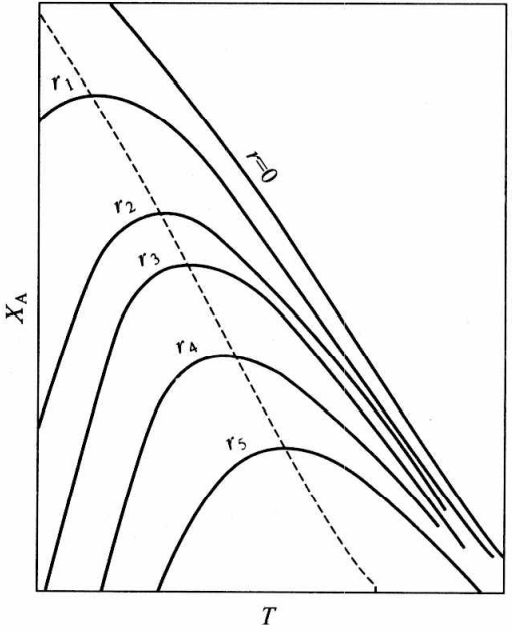
\includegraphics[width=5cm]{figs/fig2.4}}
		\centerline{\scriptsize{可逆放热反应的反应速率与温度及转化率的关系}}
		\column{7cm}
		曲线为等反应速率线，$r_5>r_4>r_3>r_2>r_1$
		\\$r=0$的曲线为平衡曲线，为反应进行的极限。
		\\连结所有等速率线上的极值点所构成的曲线(即图示虚线)，叫做最佳温度曲线。
		\\对于可逆放热反应，如果从始至终按最佳温度曲线操作，那么整个过程将以最高的反应速率进行。
	\end{columns}
\end{frame}


\begin{frame}[t]
    \frametitle{}
    \vspace{-1em}
    \begin{block}{习题2.6}
        下面是两个反应的 T-X 关系图，图中 AB 是平衡曲线 ； NP 是最佳温度曲线 ； AM 是等温线；HB 是等转化率线 。 根据下面两图回答 ：
        \begin{figure}[htpb]
            \centering
            
\includegraphics[width=.8\linewidth]{习题2.6}
        \end{figure}
        \vspace{-1em}
        \begin{enumerate}
          \item 是可逆反应还是不可逆反应？
          \item 是放热反应还是吸热反应？
        \end{enumerate}
    \end{block}
\end{frame}


\begin{frame}[t]
    \frametitle{}
    \vspace{-1em}
    \begin{block}{习题2.6}
        \begin{figure}[htpb]
            \centering
            
\includegraphics[width=.8\linewidth]{习题2.6}
        \end{figure}
        \vspace{-1em}
        \begin{enumerate}
          \item 在等温线上 ， A 、 D 、 O 、 E 、 M 点中 ， 哪点速率最大 ， 哪一点速率最小 ？
          \item 在等转化率线上 ， H 、 C 、 R 、 O 、 F 及 B 点中，哪点速率最大 ， 哪点最小 ？
          \item 在 C 、 R 两点中 ， 谁的速率大 ？
          \item 根据图中所给的十点 ， 判断哪一点速率最大 ？
        \end{enumerate}
    \end{block}
\end{frame}
\section{复合反应}


% \begin{frame}[t]
%     \frametitle{}
%     \begin{question}
%         由于存在多个化学反应，物系中任一反应组分既可能只参与其中一个反应，也可能同时参与其中若干个反应。某一反应既可能是某一反应的反应物，又可能是另一反应的反应产物。在这种情况下，该组分的转化速率该如何表示？
%         \[
%             \ch{A + B ->[k1] C} \qquad r_\mathrm{A1} = k_1c_\mathrm{A}c_\mathrm{B}
%         \]
%         \[
%             \ch{C ->[k2] A + B} \qquad r_\mathrm{A2} = k_2c_\mathrm{C}
%         \]
%     \end{question}
% \end{frame}


\begin{frame}{反应组分的消耗速率或生成速率}
	
    \begin{redblock}{A的转化速率是多少？}
        \[
            \ch{A + B ->[k1] R} \qquad r_\mathrm{A1} = k_1 c_\mathrm{A}c_\mathrm{B}
        \]
        \[
            \ch{A ->[k2] P}  \qquad r_\mathrm{A2} = k_2 c_\mathrm{A}^2
        \]
        \[
            \ch{M + N ->[k3] A} \qquad r_\mathrm{A3} = k_3c_\mathrm{M}c_\mathrm{N}
        \]
    \end{redblock}
	
    复合反应中某组份的反应量是其所参与的各个化学反应共同作用的结果。
	
    我们把单位时间内单位体积反应混合物中某一组份$i$的反应量叫做该组份的\highlight{消耗速率}($i$为反应物)或\highlight{生成速率}($i$为反应产物)，并以符号$\mathcal{R}_i$表示。
\end{frame}




\begin{frame}[t]
    \frametitle{}
    \begin{redblock}{A的转化速率是多少？}
        \[
            \ch{A + B ->[k1] R} \qquad r_\mathrm{A1} = k_1 c_\mathrm{A}c_\mathrm{B}
        \]
        \[
            \ch{A ->[k2] P}  \qquad r_\mathrm{A2} = k_2 c_\mathrm{A}^2
        \]
        \[
            \ch{M + N ->[k3] A} \qquad r_\mathrm{A3} = k_3c_\mathrm{M}c_\mathrm{N}
        \]
        \tcblower
        \[
            \mathcal{R}_\mathrm{A} = r_\mathrm{A3} - r_\mathrm{A1} - r_\mathrm{A2} = k_3c_\mathrm{M}c_\mathrm{N} - k_1 c_\mathrm{A}c_\mathrm{B} - k_2 c_\mathrm{A}^2
        \]
    \end{redblock}
    \begin{itemize}
      \item $\mathcal{R}_i$值若为正，表示该组份在反应过程中是增加的，代表生成速率；
      \item $\mathcal{R}_i$值若为负，表示该组份在反应过程中是减少的，代表消耗速率。
    \end{itemize}
\end{frame}


\begin{frame}[t]
    \frametitle{}
    \begin{question}
        如下反应网络，各物质的净反应速率是？
        \begin{center}
            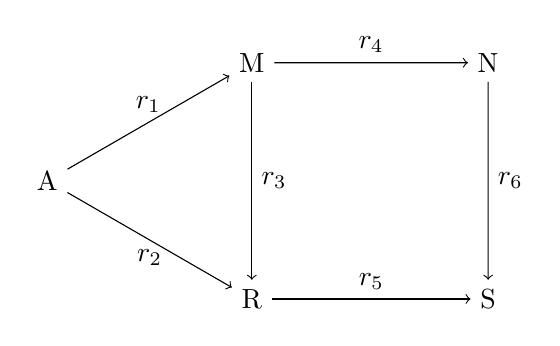
\begin{tikzpicture}[scale=1.5]
                \node (R) at (0,0) {R};
                \node (S) at (2,0) {S};
                \node (M) at (0,2) {M};
                \node (N) at (2,2) {N};
                \node (A) at (150:2) {A};
                \draw [->] (A) -- (M) node [above,midway]{$r_1$};
                \draw [->] (A) -- (R) node [below,midway]{$r_2$};
                \draw [->] (M) -- (N) node [above,midway]{$r_4$};
                \draw [->] (M) -- (R) node [right,midway]{$r_3$};
                \draw [->] (R) -- (S) node [above,midway]{$r_5$};
                \draw [->] (N) -- (S) node [right,midway]{$r_6$};
            \end{tikzpicture}
        \end{center}
    \end{question}
\end{frame}


% \begin{frame}{反应组份的转化速率和生成速率}
% 	$\mathcal{R}_i$应等于按组份$i$计算的各个反应的反应速率的代数和。
% 	$$\mathcal{R}_i=\sum_{j=1}^{M} \nu_{ij}\overline{r}_j$$
% 	\\$\overline{r}_j$为第$j$个反应式的反应速率，乘以组份$i$在第$j$个反应中的化学计量系数$\nu_{ij}$，则得按组份$i$计算的第$j$个反应的反应速率。
% 	\begin{itemize}
%       \item $\mathcal{R}_i$值若为正，表示该组份在反应过程中是增加的，代表生成速率；
%       \item $\mathcal{R}_i$值若为负，则情况相反，代表消耗速率，或转化速率。
%     \end{itemize}
	
%     $\mathcal{R}_i$与反应速率$r_i$的区别在于前者是针对若干反应，而后者则是对一个反应而言。如果只进行一个反应，$r_i=|\mathcal{R}_i|$
% \end{frame}



% \begin{frame}[t]
%     \frametitle{}
%     \begin{example}
%         对于可逆反应
%         \[
%             \ch{A + B <=>[k1][k2] C}
%         \]
%         实质上由两个反应所组成：
%         \[
%             \ch{A + B ->[k1] C} \qquad r_\mathrm{A1} = k_1c_\mathrm{A}c_\mathrm{B}
%         \]
%         \[
%             \ch{C ->[k2] A + B} \qquad r_\mathrm{A2} = k_2c_\mathrm{C}
%         \]
%         则反应组分A的净反应速率为：
%         \[
%             \mathcal{R}_\mathrm{A} = r_\mathrm{A2} - r_\mathrm{A1} = k_2c_\mathrm{C} - k_1c_\mathrm{A}c_\mathrm{B}
%         \]
%     \end{example}
% \end{frame}


\begin{frame}[t]
    \frametitle{}
    \vspace{-5pt}
    \begin{block}{例2.4}
        高温下将乙烷进行热裂解以生产乙烯，其反应及速率方程如下：
		$$\begin{array}{r}
		\ce{C2H6 <=> C2H4 + H2}\\
		\ce{2C2H6 -> C3H8 + CH4}\\
		\ce{C3H6 <=> C2H2 + CH4}\\
		\ce{C2H2 + C2H4 -> C4H6}\\
		\ce{C2H4 + C2H6 -> C3H6 + CH4}
	\end{array}~~~~~~~~~~~~
	\begin{array}{l}
		\overline{r}_1=\overrightarrow{k}_1c_\mathrm{A}-\overleftarrow{k}_1c_\mathrm{E}c_\mathrm{H}\\
		\overline{r}_2=\overrightarrow{k}_2c_\mathrm{A}\\
		\overline{r}_3=\overrightarrow{k}_3c_\mathrm{P}-\overleftarrow{k}_3c_\mathrm{R}c_\mathrm{M}\\
		\overline{r}_4=\overrightarrow{k}_4c_\mathrm{R}c_\mathrm{E}\\
		\overline{r}_5=\overrightarrow{k}_5c_\mathrm{E}c_\mathrm{A}
	\end{array}$$
    式中，下标A，R，E，P，M和H分别代表\ce{C2H6}、 \ce{C2H2}、 \ce{C2H4}、 \ce{C3H6}、 \ce{CH4}和 \ce{H2}。试导出乙烷的转化速率，乙烯的生成速率表达式。
    \tcblower
    \pause
        \[
            \mathcal{R}_\mathrm{A} = -r_\mathrm{1} - 2r_\mathrm{2} - r_\mathrm{5} = -\overrightarrow{k}_1c_\mathrm{A} + \overleftarrow{k}_1c_\mathrm{E}c_\mathrm{H} - 2\overrightarrow{k}_2c_\mathrm{A} - \overrightarrow{k}_5c_\mathrm{E}c_\mathrm{A}
        \]
        \[
            \mathcal{R}_\mathrm{E} = r_\mathrm{1} - r_\mathrm{4} - r_\mathrm{5} = \overrightarrow{k}_1c_\mathrm{A}-\overleftarrow{k}_1c_\mathrm{E}c_\mathrm{H} - \overrightarrow{k}_4c_\mathrm{R}c_\mathrm{E} - \overrightarrow{k}_5c_\mathrm{E}c_\mathrm{A}
        \]
    \end{block}
\end{frame}


\begin{frame}[t]
    \frametitle{}
    \begin{redblock}{习题2.9}
        在一恒容反应器中进行下列液相反应 ：
        \[
            \ch{A + B -> R} \qquad r_\mathrm{R} = 1.6 c_\mathrm{A}
        \]
        \[
            \ch{2 A -> D}  \qquad r_\mathrm{D} = 8.2 c_\mathrm{A}^2
        \]
        式中$r_\mathrm{R}$、$r_\mathrm{D}$分别表示产物 R 及 D 的生成速率，其单位均为 \si{kmol.m^{-3}.h^{-1}}， 反应用的原料为 A 与 B 的混合物 ， 其中 A 的浓度为 \SI{2}{kmol.m^{-3}} ， 试计算 A 的转化率达 95\%时所需要的反应时间 。
        \tcblower
        \pause
        \[
            \mathcal{R}_\mathrm{A} = -r_\mathrm{R} - 2r_\mathrm{D} = -1.6 c_\mathrm{A} - 16.4c_\mathrm{A}^2
        \]
        \[
            -\frac{\dif c_\mathrm{A}}{\dif t} = -\mathcal{R}_\mathrm{A} = 1.6 c_\mathrm{A} + 16.4 c_\mathrm{A}^2
        \]
    \end{redblock}
\end{frame}


\begin{frame}[t]
    \frametitle{}
    \vspace{-5pt}
    \begin{block}{例2.4 改}
		$$\begin{array}{r}
		\ce{C2H6 <=> C2H4 + H2}\\
		\ce{2C2H6 -> C3H8 + CH4}\\
		\ce{C3H6 <=> C2H2 + CH4}\\
		\ce{C2H2 + C2H4 -> C4H6}\\
		\ce{C2H4 + C2H6 -> C3H6 + CH4}
	\end{array}~~~~~~~~~~~~
	\begin{array}{l}
		r_1=?\\
		r_2=?\\
		r_3=?\\
		r_4=?\\
		r_5=?
	\end{array}$$
    通过实验测得\ce{C2H6}、 \ce{C2H2}、 \ce{C2H4}、 \ce{C3H6}、 \ce{CH4}和 \ce{H2}的消耗速率或生成速率$\mathcal{R}_\mathrm{A}$，$\mathcal{R}_\mathrm{R}$，$\mathcal{R}_\mathrm{E}$，$\mathcal{R}_\mathrm{P}$，$\mathcal{R}_\mathrm{M}$，$\mathcal{R}_\mathrm{H}$，如何求各反应的反应速率？
    \tcblower
    \pause
        \[
            \mathcal{R}_\mathrm{A} = -r_\mathrm{1} - 2r_\mathrm{2} - r_\mathrm{5}
        \]
        \[
            \mathcal{R}_\mathrm{E} = r_\mathrm{1} - r_\mathrm{4} - r_\mathrm{5}
        \]
    \end{block}
\end{frame}


\begin{frame}{如何得到复合反应中各反应的反应速率？}
	复合反应动力学实验测量得到的是各个反应综合的结果，即反应组分的生成速率或消耗速率。动力学研究最关心的是各个反应的反应速率，因之就存在一个如何由$\mathcal{R}_i$求$\overline{r}_j$的问题。
	\begin{itemize}
		\item 明确系统中有哪些反应，并分清主次。
		\item 忽略次要反应，只考虑起主要作用的反应。
		\item 设所要考虑的反应数目为M，通过实验测定不少于M个组分的生成速率或消耗速率。
		\item 得到M个线性代数方程，解之得各个反应的反应速率$\overline{r}_j$。
	\end{itemize}
	~~~~~~~~应注意，这M个反应必须是独立反应。所谓独立反应是指这些反应中任何一个反应都不可能由其余反应进行线性组合而得到。
\end{frame}


\begin{frame}{独立反应数的确定}
	以甲烷水蒸汽转化反应为例：
    \[
        \ch{CH4 + H2O <=> CO + 3 H2} \qquad \quad (1)
    \]
    \[
        \ch{CH4 + 2 H2O <=> CO2 + 4 H2} \qquad (2)
    \]
    \[
        \ch{CO + H2O <=> CO2 + H2} \qquad \quad \quad (3)
    \]
	其中只有两个是独立反应，因为其中总有一个反应可由其余两个线性组合得到，

    例如$(1)+(3)=(2)$
\end{frame}


\begin{frame}[fragile]
    \frametitle{通过化学计量系数矩阵得到独立反应数}
	对于化学计量系数矩阵A，其元素由全部5个反应组分在对应的3个化学反应式中的化学计量系数构成。
	$$\mathrm{CH_4~H_2~H_2O~CO~CO_2}$$
	$$\mathrm{A} = \begin{pmatrix}
	-1&  3&  -1&  -1& 0\\
	-1&  4&  -2&  0& 1\\
	0&  1&  -1&  -1& 1
\end{pmatrix}~~~~
\begin{matrix}
	(1)\\
	(2)\\
	(3)
\end{matrix}$$
	\\经初等变换后，求得矩阵A的秩$R(\mathrm{A})=2$，此时独立反应数等于矩阵的秩。
    \begin{codeblock}{使用Matlab计算矩阵A的秩}
A = [-1 3 -1 1 0; -1 4 -2 0 1; 0 1 -1 -1 1];
rank(A) # 返回结果 2
    \end{codeblock}
\end{frame}


\begin{frame}{通过原子系数矩阵得到独立反应数}
	在未知化学反应式的情况下，还可根据反应组分确定独立反应数。将反应式中所包含的全部元素种类，按分别出现在5个反应组分中的原子个数，写成原子系数矩阵B。
	$$\mathrm{CH_4~H_2~H_2O~CO~CO_2}$$
	$$\mathrm{B} = \begin{pmatrix}
		1&  0&  0&  1& 1\\
		4&  2&  2&  0& 0\\
		0&  0&  1&  1& 2
	\end{pmatrix}~~~~~~ 
	\begin{matrix}
		\mathrm{C}\\
		\mathrm{H}\\
		\mathrm{O}
	\end{matrix}$$
	\\求得矩B的秩$R(\mathrm{B})=3$，此时的独立反应数等于反应组分数$-R(\mathrm{B})$
	$$5-3=2$$
	\end{frame}


\begin{frame}{复合反应的基本类型}
	复合反应包括三个基本类型：
	\begin{itemize}
		\item 并列反应\par 反应系统中各个反应的反应组分各不相同
		\item 平行反应\par 反应物完全相同而反应产物不相同或不全相同
		\item 连串反应\par 一个反应的反应产物同时又是另一个反应的反应物
	\end{itemize}
	可逆反应亦属复合反应之列，但它可按单一反应的办法来处理，所以不将它包括在内。
\end{frame}


\begin{frame}{并列反应}
    \[
        \ch{A -> P}
    \]
    \[
        \ch{B -> Q}
    \]
	各个反应都可按单一反应来处理而得到相应的速率方程。
	
    任一个反应的反应速率不受其他反应的反应组分浓度的影响，因此，各个反应独立进行是并列反应的动力学特点。
    \begin{alertblock}
        例外情况：
        \begin{enumerate}
          \item 某些多相催化反应
          \item 变容反应
        \end{enumerate}
    \end{alertblock}
\end{frame}


\begin{frame}{平行反应}
    \[
        \ch{A -> P} \qquad r_\mathrm{P}=k_1c_\mathrm{A}^\alpha
    \]
    \[
        \ch{$\nu_\mathrm{A}$ A ->Q} \qquad r_\mathrm{Q}=k_2c_\mathrm{A}^\beta
    \]
	如果我们的目的是生产P，则P称为\highlight{目的产物}(或主产物)，其它产物均称\highlight{副产物}。
	
	生成主产物的反应称\highlight{主反应}，其它的均称为\highlight{副反应}。
	
    研究复合反应的目标之一是加快主反应的速率，降低副反应的速率，以获得尽可能多的目的产物。通常用\highlight{瞬时选择性}来评价主副反应速率相对大小。
    \[
        S=\mu_\mathrm{PA}\frac{\mathscr{R}_\mathrm{P}}{|\mathscr{R}_\mathrm{A}|}=\mu_\mathrm{PA}\frac{\mbox{目的产物的生成速率}}{|\mbox{关键反应物的消耗速率}|}
    \]
	式中，$\mu_\mathrm{PA}$为生成1molP所消耗的A的mol数。用瞬时选择性这个词，是要表明其值随反应物系的组成及温度而变，它是一个瞬时值。
\end{frame}


\begin{frame}{浓度对平行反应瞬时选择性的影响}
	\[
        S=\frac{k_1c_\mathrm{A}^\alpha}{k_1c_\mathrm{A}^\alpha+|{\nu_\mathrm{A}}|k_2c_\mathrm{A}^\beta}=\frac{1}{1+\frac{k_2}{k_1}|{\nu_\mathrm{A}}|c_\mathrm{A}^{\beta -\alpha}}
    \]
	若温度一定，则$k_1$和$k_2$为常数，反应物浓度$c_\mathrm{A}$改变时，瞬时选择性的变化与主副反应级数有关。
    \only<1>{
    \begin{itemize}
		\item  当$\alpha = \beta$时，S与浓度无关，仅为温度的函数
		\item  当$\alpha > \beta$时，反应物浓度提高，S会？？？
		\item  当$\alpha < \beta$时，反应物浓度提高，S会？？？
	\end{itemize}    
    }
    \only<2>{
    \begin{itemize}
		\item  当$\alpha = \beta$时，S与浓度无关，仅为温度的函数
		\item  当$\alpha > \beta$时，反应物浓度提高，S增加，高浓度操作有利
		\item  当$\alpha < \beta$时，反应物浓度提高，S减小，低浓度操作有利
	\end{itemize}
    }
\end{frame}


\begin{frame}{温度对平行反应瞬时选择性的影响}
	设主副反应的活化能分别为$E_1$和$E_2$，且反应速率常数$k_1$和$k_2$与温度的关系符合阿伦尼乌斯公式，则
    \[
        S=\frac{1}{1+\frac{A_2}{A_1}\exp(\frac{E_1-E_2}{RT})|{\nu_\mathrm{A}}|c_\mathrm{A}^{\beta -\alpha}}
    \]
	当浓度一定时，温度对瞬时选择性的影响取决于主副反应活化能的相对大小。
    
    \begin{itemize}
		\item 当$E_1> E_2$时，温度越高，反应的瞬时选择性越大
		\item 当$E_2> E_1$时，温度升高，反应的瞬时选择性降低
	\end{itemize}
	
\end{frame}


\begin{frame}{连串反应}
    \[
        \ch{A ->[k1] P ->[k2] Q} \qquad r_\mathrm{P} = k_1c_\mathrm{A}^\alpha - k_2c_\mathrm{P}^\beta
    \]
    \begin{itemize}
      \item 无论目的产物是P还是Q，提高反应物A的转化率总是有利的
      \item Q为目的产物时，加速这两个反应都是有利的。可采用高温高浓度的方法。
      \item 若目的产物为P，则应使第二个反应的速率尽可能的慢，以获得更多的产品P。
      \item 由于P能进一步转化成Q，因此，中间产物P必然存在一最大收率，反应进行应适可而止，不能过度。
      \item 选择有利于第一个反应而抑制第二个反应的催化剂，是提高P收率的有效方法。
    \end{itemize}
\end{frame}


\begin{frame}[t]
    \frametitle{}
    \begin{block}{例2.4}
        高温下将乙烷进行热裂解以生产乙烯，其反应及速率方程如下：
		$$\begin{array}{r}
		\ce{C2H6 <=> C2H4 + H2}\\
		\ce{2C2H6 -> C3H8 + CH4}\\
		\ce{C3H6 <=> C2H2 + CH4}\\
		\ce{C2H2 + C2H4 -> C4H6}\\
		\ce{C2H4 + C2H6 -> C3H6 + CH4}
	\end{array}~~~~~~~~~~~~
	\begin{array}{l}
		\overline{r}_1=\overrightarrow{k}_1c_\mathrm{A}-\overleftarrow{k}_1c_\mathrm{E}c_\mathrm{H}\\
		\overline{r}_2=\overrightarrow{k}_2c_\mathrm{A}\\
		\overline{r}_3=\overrightarrow{k}_3c_\mathrm{P}-\overleftarrow{k}_3c_\mathrm{R}c_\mathrm{M}\\
		\overline{r}_4=\overrightarrow{k}_4c_\mathrm{R}c_\mathrm{E}\\
		\overline{r}_5=\overrightarrow{k}_5c_\mathrm{E}c_\mathrm{A}
	\end{array}$$
    式中，下标A，R，E，P，M和H分别代表\ce{C2H6}、 \ce{C2H2}、 \ce{C2H4}、 \ce{C3H6}、 \ce{CH4}和 \ce{H2}。试导出生成乙烯的瞬时选择性表达式。
    \end{block}
\end{frame}


\begin{frame}{反应网络}
	前面介绍的复合反应的三种基本类型，各有各自的特点，实际反应系统同时兼有这三种类型的也不少见，这样复杂的反应系统，往往构成一个网络，称之为反应网络。
	\begin{columns}[c]
	\column{7cm}
	\begin{center}
		\begin{tikzpicture}[scale=1.5]
			\node (C) at (0,0) {C};
			\node (D) at (2,0) {D};
			\node (B) at (0,2) {B};
			\node (A) at (150:2) {A};
			\draw [->] (A) -- (B) node [above,midway]{1};
			\draw [->] (A) -- (C) node [above,midway]{2};
			\draw [->] (B) -- (C) node [right,midway]{3};
			\draw [->] (C) -- (D) node [above,midway]{4};
		\end{tikzpicture}
	\end{center}
	
	\column{7cm}
	\begin{itemize}
		\item 反应1，2构成平行反应
		\item 反应1，3，4构成连串反应
		\item 反应2，4构成连串反应
	\end{itemize}	
		\end{columns}
		\bigskip

		随着反应数目的增多，反应系统的动力学表征将变得越来越复杂，解决办法是将反应网络简化。
	
\end{frame}
\section{反应速率方程的变换与积分}

\begin{frame}{反应速率方程的变换}
    $$r=kc_\mathrm{A}^\alpha c_\mathrm{B}^\beta\cdots $$
    \\对于一定的反应系统，反应速率为温度及各反应组分浓度的函数。但是，在实际使用时会带来不便，因为纵使在等温情况下，各个反应组分浓度均是变量。
    \\当原料配比一定时，各个反应组分浓度可以进行变换，用一个反应变量来表示。在化学反应进行中，各反应组分浓度的变化应符合化学计量关系，因此可用关键组分的转化率或目的产物的收率来表示反应的进程。
\end{frame}


\begin{frame}{单一反应}
    $$\ce {\nu_A A + \nu_B B -> \nu_P P}$$
    $$r_\mathrm{A}=kc_\mathrm{A}^\alpha c_\mathrm{B}^\beta$$
    \\反应开始时反应混合物中不含P，组分A和B的浓度分别为$c_\mathrm{A0}$和$c_\mathrm{B0}$，若反应在等温下进行，则$k$为一常数。现要将反应速率方程变换为组分A的转化率$X_\mathrm{A}$的函数，可分两种情况进行讨论。
    \begin{itemize}
        \item[\bullet]  恒容情况
        \item[\bullet]  变容情况
    \end{itemize}
\end{frame}


\begin{frame}{单一反应，恒容情况}
    \vspace*{-10pt}
    \[
        \nu_\mathrm{A}\mathrm{A} \quad + \quad \nu_\mathrm{B}\mathrm{B} \qquad \to \qquad \nu_\mathrm{P}\mathrm{P}
    \]
    \[
        c_\mathrm{A0} \qquad \quad c_\mathrm{B0} \qquad \qquad \qquad 0
    \]
    \[
        \qquad c_\mathrm{A} \quad \quad c_\mathrm{B0} - \frac{\nu_\mathrm{B}}{\nu_\mathrm{A}}c_\mathrm{A0}X_\mathrm{A} \qquad \frac{\nu_\mathrm{P}}{\nu_\mathrm{A}}c_\mathrm{A0}X_\mathrm{A}
    \]
    恒容情况，$c_\mathrm{A}=c_\mathrm{A0}(1-X_\mathrm{A})$，$c_\mathrm{B}=c_\mathrm{B0}-\frac{\nu_\mathrm{B}}{\nu_\mathrm{A}}c_\mathrm{A0}X_\mathrm{A}$，代入速率方程，得
    $$r_\mathrm{A}=kc_\mathrm{A0}^\alpha(1-X_\mathrm{A})^\alpha (c_\mathrm{B0}-\frac{\nu_\mathrm{B}}{\nu_\mathrm{A}}c_\mathrm{A0}X_\mathrm{A})^\beta$$
    \\等式右边是单一变量$X_\mathrm{A}$的函数，左边也可用$X_\mathrm{A}$的变化来表示：
    $$r_\mathrm{A}=-\frac{\mathrm{d}c_\mathrm{A}}{\mathrm{d}t}=c_\mathrm{A0}\frac{\mathrm{d}X_\mathrm{A}}{\mathrm{d}t}$$
    $$c_\mathrm{A0}\frac{\mathrm{d}X_\mathrm{A}}{\mathrm{d}t}=kc_\mathrm{A0}^\alpha(1-X_\mathrm{A})^\alpha (c_\mathrm{B0}-\frac{\nu_\mathrm{B}}{\nu_\mathrm{A}}c_\mathrm{A0}X_\mathrm{A})^\beta$$
\end{frame}


\begin{frame}{单一反应，变容情况}
    若反应非恒容，则应考虑体积变化对摩尔浓度的影响，这时$c_\mathrm{A} \neq c_\mathrm{A0}(1-X_\mathrm{A})$。
    
    将反应前后各组分的量列出如下：
    \begin{table}
        \centering
        \begin{tabular}{ccc}
            组分 & 反应前 & 转化率为$X_\mathrm{A}$时  \\ 
            A & $n_\mathrm{A0}$ & $n_\mathrm{A0}-n_\mathrm{A0}X_\mathrm{A}$  \\ 
            B & $n_\mathrm{B0}$ & $n_\mathrm{B0}-\frac{\nu_\mathrm{B}}{\nu_\mathrm{A}}n_\mathrm{A0}X_\mathrm{A}$  \\ 
            P & 0 & $\frac{-\nu_\mathrm{P}}{\nu_\mathrm{A}}n_\mathrm{A0}X_\mathrm{A}$ \\ \toprule
            总计 & $n_\mathrm{t0}=n_\mathrm{A0}+n_\mathrm{B0}$ & $n_\mathrm{t}=n_\mathrm{t0}+n_\mathrm{A0}X_\mathrm{A}\delta_\mathrm{A}$ \\ 
        \end{tabular}
    \end{table}
    
    上表中，$\delta_\mathrm{A}=\sum \nu_i/|\nu_\mathrm{A}|$
    
    $\delta_\mathrm{A}$叫做\highlight{膨胀因子}，其物理意义是转化1molA时，反应混合物总摩尔数的变化。
    
    $\sum \nu_i$为反应产物与反应物的化学计量系数之和。
\end{frame}


\begin{frame}[t]
    \frametitle{}
    \begin{question}
        对于气相反应 A+2B→3C，计算$\delta_\mathrm{A}$的值？
        \tcblower
        A. -1

        \only<1>{
            B. 0
        }
        \only<2>{
            \red{B. 0}
        }

        C. 1

        D. 2
    \end{question}
\end{frame}


\begin{frame}[t]
    \frametitle{}
    \begin{question}
        对于气相反应 \ce{C6H6 + 3H2 -> C6H12}，计算$\delta_{C_6H_6}$的值？
        \tcblower
        A. -1

        B. 1

        \only<1>{
            C. -3
        }
        \only<2>{
            \red{C. -3}
        }

        D. 3
    \end{question}
\end{frame}


\begin{frame}[t]
    \frametitle{}
    \begin{question}
        对于气相反应 \ce{C6H6 + 3H2 -> C6H12}，计算$\delta_{H_2}$的值？
        \tcblower
        \only<1>{
            A. -1
        }
        \only<2>{
            \red{A. -1}
        }

        B. 1

        C. -3

        D. 3
    \end{question}
\end{frame}


\begin{frame}{变容情况反应速率与转化率的关系}
    如果该反应系统中气体混合物为理想气体，在恒温恒压下，有
    \[
        \begin{aligned}
             V_0/V&=n_\mathrm{t0}/n_\mathrm{t}\\
             &=n_\mathrm{t0}/(n_\mathrm{t0}+n_\mathrm{A0}X_\mathrm{A}\delta_\mathrm{A})\\
             \Longrightarrow V&=V_0(1+y_\mathrm{A0}X_\mathrm{A}\delta_\mathrm{A})
        \end{aligned}
    \]
    \begin{itemize}
      \item $\delta_\mathrm{A}>0$时，$V>V_0$
      \item $\delta_\mathrm{A}=0$时，$V=V_0$
      \item $\delta_\mathrm{A}<0$时，$V<V_0$
    \end{itemize}
\end{frame}


\begin{frame}{变容情况反应速率与转化率的关系}
    将$V=V_0(1+y_\mathrm{A0}X_\mathrm{A}\delta_\mathrm{A})$代入，得
    \[
        c_\mathrm{A}=\frac{n_\mathrm{A0}(1-X_\mathrm{A})}{V}=\frac{c_\mathrm{A0}(1-X_\mathrm{A})}{1+y_\mathrm{A0}X_\mathrm{A}\delta_\mathrm{A}}
    \]
    \[
        c_\mathrm{B}=\frac{n_\mathrm{B0}-\frac{\nu_\mathrm{B}}{\nu_\mathrm{A}}n_\mathrm{A0}X_\mathrm{A}}{V}=\frac{c_\mathrm{B0}-\frac{\nu_\mathrm{B}}{\nu_\mathrm{A}}c_\mathrm{A0}X_\mathrm{A}}{1+y_\mathrm{A0}X_\mathrm{A}\delta_\mathrm{A}}
    \]
    将上述$c_\mathrm{A},c_\mathrm{B}$代入反应速率方程可得变容情况下反应速率与转化率的关系式：
    \[
        r_\mathrm{A}=k\frac{c_\mathrm{A0}^\alpha(1-X_\mathrm{A})^\alpha (c_\mathrm{B0}-\frac{\nu_\mathrm{B}}{\nu_\mathrm{A}}c_\mathrm{A0}X_\mathrm{A})^\beta}{(1+y_\mathrm{A0}X_\mathrm{A}\delta_\mathrm{A})^{\alpha+\beta}}
    \]
    与恒容情况相比多了一个\highlight{体积校正因子}$(1+y_\mathrm{A0}X_\mathrm{A}\delta_\mathrm{A})^\mathrm{m}$，指数m由反应级数决定。
\end{frame}


\begin{frame}[t]
    \frametitle{}
    \begin{question}
        将反应速率方程变换为转化率函数的主要目的是什么？
        \tcblower
        A. 简化温度对反应速率的影响

        \only<1>{
            B. 消除浓度变量，便于工程计算
        }
        \only<2>{
            \red{B. 消除浓度变量，便于工程计算}
        }

        C. 增加反应级数的复杂性

        D. 忽略化学计量关系
    \end{question}
\end{frame}


\begin{frame}{变容情况反应速率与转化率的关系}
    \[
        r_\mathrm{A}=k\frac{c_\mathrm{A0}^\alpha(1-X_\mathrm{A})^\alpha (c_\mathrm{B0}-\frac{\nu_\mathrm{B}}{\nu_\mathrm{A}}c_\mathrm{A0}X_\mathrm{A})^\beta}{(1+y_\mathrm{A0}X_\mathrm{A}\delta_\mathrm{A})^{\alpha+\beta}}
    \]
    若将变容情况下的$r_\mathrm{A} = -\frac{1}{V}\frac{\dif n_\mathrm{A}}{\dif t}$变为转化率的函数，
    \[
        r_\mathrm{A} = \frac{-1}{V_0(1+y_\mathrm{A0}X_\mathrm{A}\delta_\mathrm{A})}\frac{\mathrm{d}(n_\mathrm{A0}-n_\mathrm{A0}X_\mathrm{A})}{\mathrm{d}t}=\frac{c_\mathrm{A0}}{1+y_\mathrm{A0}X_\mathrm{A}\delta_\mathrm{A}}\frac{\mathrm{d}X_\mathrm{A}}{\mathrm{d}t}
    \]
    与恒容情况相比，也是多了一个体积校正因子。

    两式联立可得变容情况转化率与反应时间的关系：
    \[
        \frac{c_\mathrm{A0}}{1+y_\mathrm{A0}X_\mathrm{A}\delta_\mathrm{A}}\frac{\mathrm{d}X_\mathrm{A}}{\mathrm{d}t} = k\frac{c_\mathrm{A0}^\alpha(1-X_\mathrm{A})^\alpha (c_\mathrm{B0}-\frac{\nu_\mathrm{B}}{\nu_\mathrm{A}}c_\mathrm{A0}X_\mathrm{A})^\beta}{(1+y_\mathrm{A0}X_\mathrm{A}\delta_\mathrm{A})^{\alpha+\beta}}
    \]
    当$\delta_\mathrm{A}=0$时，上式便化为恒容情况下的公式$c_\mathrm{A0}\frac{\mathrm{d}X_\mathrm{A}}{\mathrm{d}t}=kc_\mathrm{A0}^\alpha(1-X_\mathrm{A})^\alpha (c_\mathrm{B0}-\frac{\nu_\mathrm{B}}{\nu_\mathrm{A}}c_\mathrm{A0}X_\mathrm{A})^\beta$。
\end{frame}


\begin{frame}{反应物系组成的变换方法}
    以浓度表示反应物系组成时的变换方法：
    \[
        c_i=\frac{c_{i0}-\frac{\nu_i}{\nu_\mathrm{A}}c_\mathrm{A0}X_\mathrm{A}}{1+y_\mathrm{A0}X_\mathrm{A}\delta_\mathrm{A}}
    \]
    此式对恒容和变容、反应物和反应产物都适用。

    以分压表示反应气体组成时：
    \[
        p_i=\frac{p_{i0}-\frac{\nu_i}{\nu_\mathrm{A}}p_\mathrm{A0}X_\mathrm{A}}{1+y_\mathrm{A0}X_\mathrm{A}\delta_\mathrm{A}}
    \]
    以摩尔分数表示反应气体组成时：
    \[
        y_i=\frac{y_{i0}-\frac{\nu_i}{\nu_\mathrm{A}}y_\mathrm{A0}X_\mathrm{A}}{1+y_\mathrm{A0}X_\mathrm{A}\delta_\mathrm{A}}
    \]
\end{frame}


\begin{frame}
    \frametitle{恒容、变容情况的判定}
    \begin{enumerate}
      \item 液相反应一般都可按恒容过程处理；
      \item 对于间歇操作，无论液相还是气相反应，总是恒容过程；
      \item 对于等温流动操作，总摩尔数不发生变化的气相反应也属于恒容过程。
    \end{enumerate}
\end{frame}


% \begin{frame}{变容情况转化率与反应时间的关系}
%     以$\ce {A + B -> P}$为例，且该反应对A及B均为一级，则
%     $$\frac{c_\mathrm{A0}}{1-y_\mathrm{A0}X_\mathrm{A}}\frac{\mathrm{d}X_\mathrm{A}}{\mathrm{d}t}=k\frac{c_\mathrm{A0}(1-X_\mathrm{A})(c_\mathrm{B0}-c_\mathrm{A0}X_\mathrm{A})}{(1-y_\mathrm{A0}X_\mathrm{A}\delta_\mathrm{A})^2}$$
%     \\化简后积分得，
%     $$t=\frac{1}{k}[\frac{1+c_\mathrm{B0}y_\mathrm{A0}/c_\mathrm{A0}}{c_\mathrm{B0}-c_\mathrm{A0}}\ln(1-\frac{c_\mathrm{A0}X_\mathrm{A}}{c_\mathrm{B0}})+\frac{1+y_\mathrm{A0}}{c_\mathrm{B0}-c_\mathrm{A0}}\ln\frac{1}{1-X_\mathrm{A}}]$$
%     \\这便是二级反应的转化率与反应时间的关系式。只有速率方程的形式较为简单时才能解析积分，多数需要采用数值积分。
% \end{frame}


\begin{frame}[t]{}
    \begin{block}{例2.5}
    \[
        \ce{C6H6 + 3H2 -> C6H12}
    \]
    已知在镍催化剂上进行苯气相加氢反应的动力学方程为
    \[
        r_\mathrm{B}=\frac{kp_\mathrm{B}p_\mathrm{H}^{0.5}}{1+Kp_\mathrm{B}}
    \]
    式中$p_\mathrm{B}$及$p_\mathrm{H}$依次为苯及氢的分压，$k$和$K$为常数。若反应气体的起始组成中不含环己烷，苯及氢的摩尔分数分别为$y_\mathrm{B0}$和$y_\mathrm{H0}$  。反应系统的总压为$p$，试将动力学方程变换为苯的转化率的$X_\mathrm{B}$函数。
    \tcblower
    \pause
    \[
        r_\mathrm{B} = k\left(p\frac{y_{B0}-y_\mathrm{B0}X_\mathrm{B}}{1-3y_\mathrm{B0}X_\mathrm{B}}\right)\left(p\frac{y_{H0}-3y_\mathrm{B0}X_\mathrm{B}}{1-3y_\mathrm{B0}X_\mathrm{B}}\right)^{0.5}\bigg/\left(1+Kp\frac{y_{B0}-y_\mathrm{B0}X_\mathrm{B}}{1-3y_\mathrm{B0}X_\mathrm{B}}\right)
    \]
    \end{block}
\end{frame}


\begin{frame}[t]{}
    \begin{redblock}{例2.5 改}
        $$\ce{C6H6 + 3H2 -> C6H12}$$
    $$(\mathrm{B})~~~~~~~~(\mathrm{H})~~~~~~~~~~~~~(\mathrm{C})~~$$
    已知在镍催化剂上进行苯气相加氢反应的动力学方程为
    \[
        r_\mathrm{B}=\frac{kp_\mathrm{B}p_\mathrm{H}^{0.5}}{1+Kp_\mathrm{B}}
    \]
    式中$p_\mathrm{B}$及$p_\mathrm{H}$依次为苯及氢的分压，$k$和$K$为常数。若反应气体的起始组成中不含环己烷，苯及氢的摩尔分数分别为$y_\mathrm{B0}$和$y_\mathrm{H0}$  。反应系统的总压为$p$，
    
    \red{试将动力学方程变换为氢的转化率的$X_\mathrm{H}$函数。}
    \end{redblock}
\end{frame}


\begin{frame}[t]
    \frametitle{}
    \begin{block}{习题2.11}
        在210℃等温下进行亚硝酸乙酯的气相分解反应
        \[
            \ch{C2H5NO2 -> NO + 0.5 CH3CHO + 0.5 C2H5OH}
        \]
        该反应为一级不可逆反应，$k = 1.39\times 10^{14}\exp(-18973/T)$，\si{s^{-1}}。
        
        (1) 若反应是在恒容下进行，系统的起始总压为\SI{0.1013}{MPa}，采用的是纯亚硝酸乙酯，试计算亚硝酸乙酯的分解率为80\%时，亚硝酸乙酯的分解速率及乙醇的生成速率。

        (2) 若采用恒压反应，乙醇的生成速率是多少？
    \end{block}
\end{frame}


\begin{frame}[t]
    \frametitle{}
    \begin{question}
        在恒压反应系统中，乙醇生成速率与恒容情况的差异主要源于？
        \tcblower
        A. 温度变化

        \only<1>{
            B. 体积膨胀导致的浓度变化
        }
        \only<2>{
            \red{B. 体积膨胀导致的浓度变化}
        }

        C. 催化剂失活

        D. 副反应的增加
    \end{question}
\end{frame}


\begin{frame}[t]
    \frametitle{}
    \begin{question}
        在恒压反应系统中，乙醇生成速率与恒容情况的差异是？
        \tcblower
        A. 恒压乙醇生成速率>恒容乙醇生成速率

        \only<1>{
            B. 恒压乙醇生成速率<恒容乙醇生成速率
        }
        \only<2>{
            \red{B. 恒压乙醇生成速率<恒容乙醇生成速率}
        }
    \end{question}
\end{frame}


\begin{frame}{复合反应}
    反应系统中同时进行数个化学反应时，亦可仿照单一反应的处理方法对速率方程作变换。设气相反应系统中含有N个反应组分，它们之间共进行M个化学反应，各个反应的反应进度为$\xi_j$。为了数学上处理方便，将这些化学反应式写成代数式的形式：
    $$\nu_{11}\mathrm{A_1}+\nu_{21}\mathrm{A_2}+\cdots+\nu_{N1}\mathrm{A_N} = 0$$
    $$\nu_{12}\mathrm{A_1}+\nu_{22}\mathrm{A_2}+\cdots+\nu_{N2}\mathrm{A_N} = 0$$
    $$\cdots \cdots$$
    $$\nu_{1M}\mathrm{A_1}+\nu_{2M}\mathrm{A_2}+\cdots+\nu_{NM}\mathrm{A_N} = 0$$
\end{frame}


\begin{frame}{复合反应}
    将组分$i$在各个反应中的反应量相加，即得该组分的总反应量
    $$n_i-n_{i0}=\sum_{j=1}^{M}\nu_{ij}\xi_j$$
    \\将所有反应组分的反应量相加，则得整个系统的总摩尔数变化
    $$n_\mathrm{t}-n_\mathrm{t0}=\sum_{i=1}^{N}\sum_{j=1}^{M}\nu_{ij}\xi_j$$
    \\代入$V/V_0=n_\mathrm{t}/n_\mathrm{t0}$整理，得
    $$c_i=\frac{n_i}{V}=\frac{n_{i0}+\sum_{j=1}^{M}\nu_{ij}\xi_j}{V_0(1+\frac{1}{n_\mathrm{t0}}\sum_{i=1}^{N}\sum_{j=1}^{M}\nu_{ij}\xi_j)}$$
\end{frame}


\begin{frame}[t]
    \frametitle{}
    \begin{redblock}{小组讨论：根据$c_i$推导计算$p_i$的公式}
        \[
            c_i=\frac{n_i}{V}=\frac{n_{i0}+\sum_{j=1}^{M}\nu_{ij}\xi_j}{V_0(1+\frac{1}{n_\mathrm{t0}}\sum_{i=1}^{N}\sum_{j=1}^{M}\nu_{ij}\xi_j)}
        \]
        \tcblower
        提示1：理想气体方程

        提示2：化简，结果中用总压$p$表示
    \end{redblock}
\end{frame}


\begin{frame}[t]{}
    \begin{block}{例2.6}
        在常压和898K下进行乙苯催化脱氢反应：
    
        $(1)~~~~\ce{C6H5C2H5 <=> C6H5-CH=CH2 + H2}$
    
        $(2)~~~~\ce{C6H5C2H5 -> C6H6 + C2H4}$
    
        $(3)~~~~\ce{C6H5C2H5 + H2 -> C6H5CH3 + CH4}$
    
        为简便起见，以A，B，T，H及S分别代表乙苯，苯，甲苯，氢及苯乙烯，在反应温度及压力下，上列各反应的速率方程为
    $$\begin{array}{l}
        r_{1}=0.1283\left(p_{\mathrm{A}}-p_{\mathrm{S}} p_{\mathrm{H}} / 0.04052\right) \qquad\mathrm{kmol/(kg·h)}\\
        r_{2}=5.745 \times 10^{-3} p_{\mathrm{A}} \qquad\mathrm{kmol/(kg·h)}\\
        r_{3}=0.2904 p_{\mathrm{A}} p_{\mathrm{H}} \qquad\mathrm{kmol/(kg·h)}
    \end{array}$$
    \vspace{-1em}

    压力的单位用MPa，进料中含乙苯10\%和$\mathrm{H_2O}$ 90\%。当苯乙烯，苯及甲苯的收率分别为60\%，0.5\%及1\%时，试计算乙苯的转化速率。
    \end{block}
\end{frame}
\section{多相催化与吸附}

\begin{frame}{多相催化}
    要使化学反应在工业上得以实现，大多数都要通过催化作用。不是使用均相催化就是使用多相催化的方式。后者的实质就是用固体催化剂来加速化学反应的进行，而反应是在催化剂的表面上发生的，因之研究反应组分在催化剂表面的吸附具有十分重要的意义。

    学习目标：
    \begin{itemize}
      \item 通过来自实验或者理论计算的动力学数据，在分子水平上描述化学反应包含的所有基元步骤。
      \item 通过微观动力学分析得到反应中间产物的表面覆盖率，从而获得基元反应速率，最终确定反应的主要反应路径和速率控制步骤。
    \end{itemize}
\end{frame}


\begin{frame}
    \frametitle{催化剂的作用}
    \begin{enumerate}
      \item 改变反应途径，降低反应所需活化能。
      \item 定向作用，改善反应的选择性。
    \end{enumerate}
    \bigskip

    \begin{minipage}{0.38\linewidth}
        \begin{figure}[htpb]
            \centering
            
\includegraphics[width=.9\linewidth]{催化剂改变途径}
        \end{figure}
    \end{minipage}\hfill
    \begin{minipage}{0.58\linewidth}
        \begin{block}{乙醇分解反应}
            \[
                \ch{C2H5OH ->[$\gamma$-Al2O3] C2H4 + H2O}
            \]
            \[
                \ch{C2H5OH ->[Cu] CH3CHO + H2}
            \]
        \end{block}
    \end{minipage}
\end{frame}


\begin{frame}{固体催化剂}
    固体催化剂绝大多数为颗粒状，一般情况下，固体催化剂由三部分组成：
    \begin{itemize}
      \item 主催化剂：起催化作用，常用的是金属和金属氧化物。
      \item 助催化剂：含量一般很少，作用是提高催化剂的催化活性、选择性和稳定性。
      \item 载体：多孔结构，增大表面积
    \end{itemize}
    
    \begin{blankblock}{}
        不同的反应对比表面有不同的要求。比表面大就意味着载体的孔半径小，从而增大了扩散阻力。
        \begin{itemize}
          \item $\alpha$-\ch{Al2O3} \quad $1\sim 10$ \si{m^2/g}。
          \item $\gamma$-\ch{Al2O3}  \quad  $100\sim 300$ \si{m^2/g}。
          \item 活性炭 \quad \ $500\sim 1500$ \si{m^2/g}。
        \end{itemize}
    \end{blankblock}
\end{frame}


\begin{frame}
    \frametitle{固体催化剂孔结构参数}
    \begin{minipage}{0.48\linewidth}
        \begin{itemize}
          \item 孔容
          \item 孔径
          \item 孔径分布
          \item 孔隙率
          \item 平均孔径
        \end{itemize}
    \end{minipage}\hfill
    \begin{minipage}{0.48\linewidth}
        \begin{figure}[htpb]
            \centering
            
\includegraphics[width=\linewidth]{固体催化剂}
        \end{figure}
    \end{minipage}
\end{frame}


\begin{frame}{多相催化反应步骤}
    \begin{columns}[c]
        \column{6.75cm}
        设多相催化反应\ce{A + B <=> R}由下列步骤所构成
        \begin{itemize}
            \item[1] 吸附 $\ce{A + {$\sigma$} <=> A{$\sigma$}}$
            \item[2] 吸附 $\ce{B + {$\sigma$} <=> B{$\sigma$}}$
            \item[3] 反应 $\ce{A{$\sigma$} + B{$\sigma$} <=> R{$\sigma$} + {$\sigma$}}$
            \item[4] 脱附 $\ce{R{$\sigma$} <=> R + {$\sigma$}}$
        \end{itemize}
        式中，$\sigma$ 表示吸附位，$\mathrm{A}\sigma$、$\mathrm{B}\sigma$、$\mathrm{R}\sigma$分别表示吸附态的A、B及R。
        \column{6.75cm}
        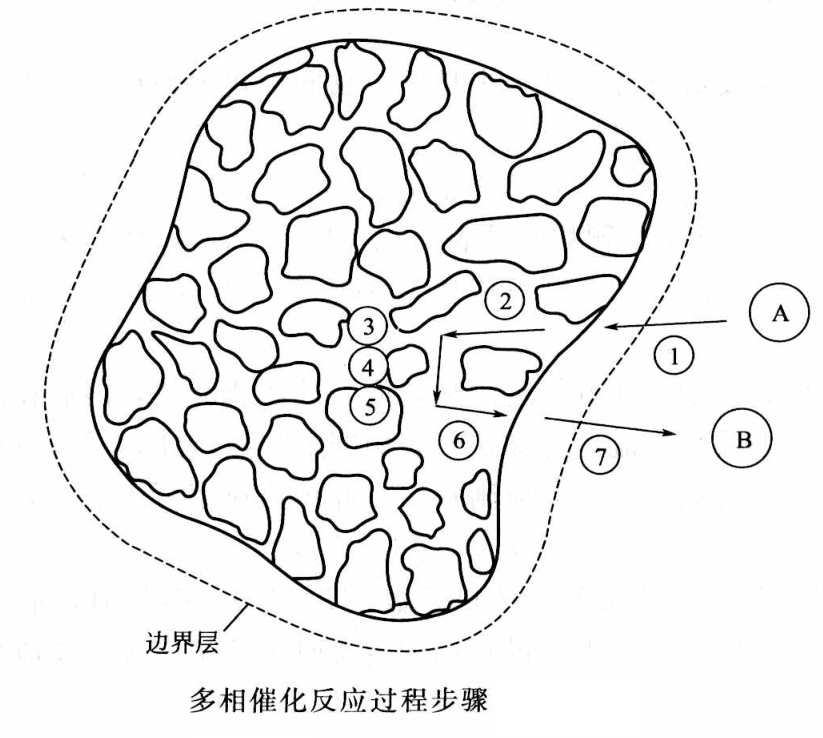
\includegraphics[width=6.75cm]{figs/fig6.1.png}
    \end{columns}
\end{frame}


\begin{frame}{物理吸附与化学吸附}
    气体在固体表面上的吸附，可分为物理吸附和化学吸附两种类型。研究固体表面的吸附是研究多相催化反应动力学的重要基础之一。
    \begin{table}        
            \caption{物理吸附与化学吸附的比较}
            \begin{tabular}{cll}
                \Xhline{1pt}
                项目 & \makecell[c]{物理吸附} & \makecell[c]{化学吸附}\\
                \hline
                吸附力 & 分子间引力 & 化学键力\\
                选择性 & 所有气体都可被吸附 & 不是所有气体都可被吸附\\
                温度 & 低温，温度升高吸附量减小 & 高温，温度升高吸附速率增加\\
                吸附热 & $8\sim 25\si{kJ.mol^{-1}}$ & $40\sim 200\si{kJ.mol^{-1}}$\\
                覆盖度 & 多层吸附 &单层吸附 \\
                应用 & 测定固体表面积及孔径大小 & 测定表面浓度，吸附和解吸速率\\
                \Xhline{1pt}
            \end{tabular}        
    \end{table}
\end{frame}


\begin{frame}{理想吸附模型}
    对固体表面上的化学吸附作定量处理时，需建立适当的吸附模型。最简单常用的是理想吸附模型，是由朗格缪尔(Langmuir)首先提出的，又称朗格缪尔吸附模型。该模型基于如下基本假设：
    \begin{enumerate}
        \item 催化剂表面各处的吸附能力是均匀的，各吸附位具有相同的能量
        \item 被吸附物仅形成单分子层吸附
        \item 被吸附分子间不发生相互作用 
    \end{enumerate}
    气体分子在催化剂表面的吸附速率与单位时间内碰撞到催化剂自由表面上的气体分子数目成正比。气体分子对表面的碰撞速率与气体的分压成正比。因吸附在自由表面进行，故又同自由表面占比成正比。
\end{frame}


\begin{frame}{单分子吸附}
    设气体A被催化剂的吸附位$\sigma$吸附
    $$\ce{A + {$\sigma$} <=>[k_a][k_d] A{$\sigma$}}$$
    
    吸附速率方程为：
    \[
        r_\mathrm{a}=k_\mathrm{a}p_\mathrm{A}(1-\theta_\mathrm{A})
    \]
    式中，$\theta_\mathrm{A}$为吸附分子A覆盖的表面所占的百分比，称为\highlight{表面覆盖率}。由于化学吸附是单层的，所以未被吸附分子占据的自由表面占比等于$(1-\theta_\mathrm{A})$，叫未覆盖率。
    
    脱附速率：
    \[
        r_\mathrm{d}=k_\mathrm{d}\theta_\mathrm{A}
    \]
    吸附的净速率：
    \[
        r=k_\mathrm{a}p_\mathrm{A}(1-\theta_\mathrm{A})-k_\mathrm{d}\theta_\mathrm{A}
    \]
   
\end{frame}


\begin{frame}{表面覆盖率与压力的关系}
        \[
            r=k_\mathrm{a}p_\mathrm{A}(1-\theta_\mathrm{A})-k_\mathrm{d}\theta_\mathrm{A}
        \]
        当吸附达到平衡时，$r=0$，则有
        \[
            \theta_\mathrm{A}=\frac{K_\mathrm{A}p_\mathrm{A}}{1+K_\mathrm{A}p_\mathrm{A}}
        \]
        上式即为理想吸附等温方程（$T$一定，描述$p$与$\theta$的关系的方程），也叫朗格缪尔吸附等温式。式中，$K_\mathrm{A}=k_\mathrm{a}/k_\mathrm{d}$，叫做吸附平衡常数，表示气体分子被吸附的强弱。
        \begin{itemize}
          \item $p$升高，覆盖率增加；
          \item 对弱吸附，$K_\mathrm{A}p_\mathrm{A}\ll1$，$\theta_\mathrm{A}=K_\mathrm{A}p_\mathrm{A}$
          \item 对强吸附，$K_\mathrm{A}p_\mathrm{A}\gg1$，$\theta_\mathrm{A}=1$
        \end{itemize}
\end{frame}


\begin{frame}
    \frametitle{表面覆盖率与温度的关系}
    \begin{minipage}{0.48\linewidth}
        \[
            k_\mathrm{a}=A_1\exp(-E_\mathrm{a}/RT)
        \]
        \[
            k_\mathrm{d}=A_2\exp(-E_\mathrm{d}/RT)
        \]
        吸附平衡常数与温度的关系为：
    \[
        K_\mathrm{A}=\frac{k_\mathrm{a}}{k_\mathrm{d}}=K_\mathrm{A0}\exp(q/RT)
    \]
    \begin{itemize}
      \item $q=E_\mathrm{d}-E_\mathrm{a}$，为吸附热
      \item 催化过程$E_\mathrm{d}>E_\mathrm{a}$，$q>0$
      \item $T$升高，$K_\mathrm{A}$下降，覆盖率减少。
    \end{itemize}
    \end{minipage}\hfill
    \begin{minipage}{0.48\linewidth}
        \begin{figure}[htpb]
            \centering
            
\includegraphics[width=\linewidth]{fig2.66.png}
            \caption{Langmuir吸附等温线($T_1<T_2<T_3$)} 
        \end{figure}
    \end{minipage}
\end{frame}
% 文献《温度对Langmuir吸附常数影响的实验研究》：脱附活化能大于吸附活化能


% \begin{frame}
%     \frametitle{六种吸附等温线}
%     \begin{figure}[htpb]
%         \centering
%         
\includegraphics[width=.67\linewidth]{吸附等温线}
%         \caption{I:Langmuir单分子层吸附 \quad II \& III:多分子层吸附 \quad IV \& V:毛细孔凝聚理论 \quad VI:其它}
%     \end{figure}
% \end{frame}


\begin{frame}{多分子吸附}
    设分子A和B同时吸附在催化剂表面上
    % \[
    %     \ce{A + B + {$2\sigma$} <=>[k_a][k_d] A{$\sigma$} + B{$\sigma$}}
    % \]
    \[
        \ce{A + {$\sigma$} <=>[k_{aA}][k_{dA}] A{$\sigma$}}
    \]
    \[
        \ce{B + {$\sigma$} <=>[k_{aB}][k_{dB}] B{$\sigma$}}
    \]
    \[
        r_\mathrm{aA}=k_\mathrm{aA}p_\mathrm{A}(1-\theta_\mathrm{A}-\theta_\mathrm{B}) \text{；}r_\mathrm{dA}=k_\mathrm{dA}\theta_\mathrm{A}
    \]
    \[
        r_\mathrm{aB}=k_\mathrm{aB}p_\mathrm{B}(1-\theta_\mathrm{A}-\theta_\mathrm{B}) \text{；}r_\mathrm{dB}=k_\mathrm{dB}\theta_\mathrm{B}
    \]
    当吸附达到平衡时，$r_\mathrm{aA}=r_\mathrm{dA}$，$r_\mathrm{aB}=r_\mathrm{dB}$
    
    联立求解可得
    \[
        \theta_\mathrm{A}=\frac{K_\mathrm{A}p_\mathrm{A}}{1+K_\mathrm{A}p_\mathrm{A}+K_\mathrm{B}p_\mathrm{B}}\text{；}\theta_\mathrm{B}=\frac{K_\mathrm{B}p_\mathrm{B}}{1+K_\mathrm{A}p_\mathrm{A}+K_\mathrm{B}p_\mathrm{B}}\text{；}\theta_\mathrm{V}=\frac{1}{1+K_\mathrm{A}p_\mathrm{A}+K_\mathrm{B}p_\mathrm{B}}
    \]
\end{frame}


\begin{frame}{解离吸附}
    在吸附过程中，会发生吸附分子解离为原子的情况，这些原子各占据一个吸附位，例如
    $$\ce{A2 + {$2\sigma$} <=>[k_a][k_d] 2A{$\sigma$}}$$
    $$r_\mathrm{a}=k_\mathrm{a}p_\mathrm{A}(1-\theta_\mathrm{A})^2$$
    $$r_\mathrm{d}=k_\mathrm{d}\theta_\mathrm{A}^2$$
    $$r=k_\mathrm{a}p_\mathrm{A}(1-\theta_\mathrm{A})^2-k_\mathrm{d}\theta_\mathrm{A}^2$$
    \\达到平衡时，净速率为零，则有
    $$\theta_\mathrm{A}=\frac{\sqrt{K_\mathrm{A}p_\mathrm{A}}}{1+\sqrt{K_\mathrm{A}p_\mathrm{A}}} \text{~~~~(朗格缪尔解离吸附等温方程)}$$
\end{frame}


\begin{frame}[t]
    \frametitle{}
    \begin{redblock}{写出丁烯异构反应\ch{A -> R}各步的净反应速率}
        \begin{minipage}{0.48\linewidth}
            \only<1>{
                \begin{enumerate}
              \item \ce{A + $\sigma$ <=>[k_{aA}][k_{dA}]A$\sigma$}
              
              \phantom{需要占位的文本}

              \item \ce{A$\sigma$ <=>[k_+][k_-] R$\sigma$}
              
              \phantom{需要占位的文本}
              \item \ce{R$\sigma$ <=>[k_{dR}][k_{aR}] R + $\sigma$}
              
              \phantom{需要占位的文本}
            \end{enumerate}
            }
            \only<2>{
                \begin{enumerate}
              \item \ce{A + $\sigma$ <=>[k_{aA}][k_{dA}]A$\sigma$}
              
              \red{$r_1 = k_\mathrm{aA} p_\mathrm{A} \theta_\mathrm{v} - k_\mathrm{dA} \theta_\mathrm{A}$}

              \item \ce{A$\sigma$ <=>[k_+][k_-] R$\sigma$}
              
              \red{$r_2 = k_+ \theta_\mathrm{A} - k_- \theta_\mathrm{R}$}

              \item \ce{R$\sigma$ <=>[k_{dR}][k_{aR}] R + $\sigma$}
              
              \red{$r_3 = k_\mathrm{dR} \theta_\mathrm{R} - k_\mathrm{aR} p_\mathrm{R} \theta_\mathrm{v}$}
            \end{enumerate}
            }
        \end{minipage}\hfill
        \begin{minipage}{0.48\linewidth}
            \begin{figure}[htpb]
                \centering
                
\includegraphics[width=\linewidth]{丁烯异构反应}
            \end{figure}
        \end{minipage}
    \end{redblock}
\end{frame}


\begin{frame}{真实吸附}
    不满足理想吸附条件的吸附，都称之为真实吸附。以焦姆金(Temkin)和弗列因特利希(Freundlich)为代表提出不均匀表面吸附理论，真实吸附模型认为固体表面是不均匀的，各吸附中心的能量不等，有强有弱。吸附时吸附分子首先占据表面活性最高的吸附中心，属强吸附，放出的吸附热大。随后，吸附越来越弱，放出的吸附热越来越小。
    \\吸附活化$E_\mathrm{a}$能随着覆盖率的增加而线性增加，脱附活化能$E_\mathrm{d}$则随着覆盖率的增加而线性降低。
    $$E_\mathrm{a}=E_\mathrm{a}^0 + \alpha\theta_\mathrm{A}$$
    $$E_\mathrm{d}=E_\mathrm{d}^0 - \beta\theta_\mathrm{A}$$    
    式中，$E_\mathrm{a}^0$和$E_\mathrm{d}^0$分别为覆盖率等于零时的吸附活化能和脱附活化能。
\end{frame}

\begin{frame}{焦姆金吸附等温式}
    吸附热
    $$q=E_\mathrm{d}-E_\mathrm{a}=(E_\mathrm{d}^0-E_\mathrm{a}^0)-(\alpha+\beta)\theta_\mathrm{A}=q_0-\gamma\theta_\mathrm{A}$$
    \\式中，$q_0=E_\mathrm{d}^0-E_\mathrm{a}^0$，$\gamma=\alpha+\beta$。导出吸附及脱附速率方程为：
    \[
        r_\mathrm{a}=k_\mathrm{a0}p_\mathrm{A}\exp(-\alpha\theta_\mathrm{A}/RT)
    \]
    \[
        r_\mathrm{d}=k_\mathrm{d0}\exp(\beta\theta_\mathrm{A}/RT)
    \]
    吸附达到平衡时，$r_\mathrm{a}-r_\mathrm{d}=0$，有
    $$\theta_\mathrm{A}=\frac{RT}{\alpha+\beta}\ln(K_\mathrm{0}p_\mathrm{A})$$
    \\上式即为真实吸附等温方程，也叫焦姆金吸附等温式。式中$K_\mathrm{0}=k_\mathrm{a0}/k_\mathrm{d0}$。此式适用于中等覆盖率的情况。
\end{frame}


\begin{frame}{弗列因特利希吸附等温式}
    弗列因特利希吸附等温式最初作为经验式提出，后来假定吸附与脱附活化能和$\ln \theta_\mathrm{A}$呈线性关系，从而从理论上推导出来
    $$\theta_\mathrm{A}=Kp_\mathrm{A}^\mathrm{m}\qquad (m<1)$$
    
    无论是焦姆金还是弗列因特利希等温式，都有其不足。
    
    对于前者，当$p_\mathrm{A}=0$时，$\theta_\mathrm{A}$却不等于零，这是不符合实际的，而后者则满足$p_\mathrm{A}=0\text{，}\theta_\mathrm{A}=0$的要求。但当$p_\mathrm{A}$增大时，后者算出的$\theta_\mathrm{A}$值可能大于1，显然这也是不合理的。
    
    因此，根据不同的模型假设可以得到不同的吸附等温方程，具体应用时必须注意实际过程是否符合或接近所选模型的假设条件，并经过实验验证。
\end{frame}


\section{多相催化反应动力学}

\begin{frame}[t]
    \frametitle{多相催化反应动力学}
    \begin{question}
        从反应工程的观点看，多相催化反应的动力学研究，其首要问题是找出反应速率方程。如何从所确定的反应步骤导出多相催化反应的总包速率方程？
    \end{question}
    要从各反应步骤的速率中导出总包速率方程，需要作出一些简化假定：
    \begin{enumerate}
      \item 定态近似
      \item 速率控制步骤
    \end{enumerate}
\end{frame}


\begin{frame}{定态近似}
    \begin{columns}[c]
        \column{7cm}
            若反应过程达到定态，中间化合物的浓度就不随时间变化，即
            $$\frac{\mathrm{d}c_\mathrm{I}}{\mathrm{d}t}=0$$
            式中，$c_\mathrm{I}$为中间化合物的浓度。
            \\也可以说，若达到定态，则串联进行的各反应步骤速率相等。
            \\这两种说法是一样的。
            $$$$
        \column{7cm}
            设化学反应$\ce{A <=> R}$由下列两个步骤构成
            $$\mathrm{A} \rightleftharpoons \mathrm{A∗} \qquad r_1=\overrightarrow{k}_1c_\mathrm{A}-\overleftarrow{k}_1c_\mathrm{A}$$
            $$\mathrm{A∗} \rightleftharpoons \mathrm{R} \qquad r_2=\overrightarrow{k}_2c_\mathrm{A}-\overleftarrow{k}_2c_\mathrm{A}$$
            中间化合物$\mathrm{A∗}$的浓度变化速率为
            \[
                \begin{aligned}
                    \frac{\mathrm{d}c_\mathrm{A∗}}{\mathrm{d}t}&=r_1-r_2 \\
                    &=(\overrightarrow{k}_1c_\mathrm{A}-\overleftarrow{k}_1c_\mathrm{A})-(\overrightarrow{k}_2c_\mathrm{A}-\overleftarrow{k}_2c_\mathrm{A})
                \end{aligned}
            \] 
    \end{columns}
\end{frame}


\begin{frame}{速率控制步骤}
    \begin{columns}[c]
        \column{7cm}
        仍以反应$\ce{A <=> R}$为例
        \\各反应步骤均为可逆反应，各反应速率的相对大小如图所示。各反应步骤的正逆反应速率是不相等的，但根据定态近似的假设，其净速率应相等，且等于反应$\ce{A <=> R}$的速率。即$$r_1=r_2=r$$
        \\第一个反应步骤接近平衡的程度$\frac{\overrightarrow{r}_1-\overleftarrow{r}_1}{\overrightarrow{r}_1}$，远较第二个步骤大，此时第二个步骤便可视为速率控制步骤。
        \column{7cm}
        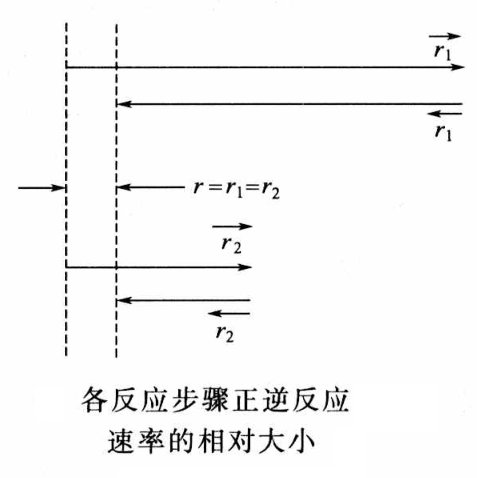
\includegraphics[width=6cm]{figs/fig2.5.png}
    \end{columns}    
\end{frame}


\begin{frame}{多相催化反应速率方程}
    以反应\ce{A + B <=> R}及如下假定的反应式为例
    \bigskip

        \begin{minipage}{0.08\linewidth}
            
        \end{minipage}\hfill
        \begin{minipage}{0.88\linewidth}
            \begin{itemize}
                \item[\highlight{A吸附}]  $\ce{A + {$\sigma$} <=> A{$\sigma$}}$ \qquad ~~~~\qquad $r_1=k_\mathrm{aA}p_\mathrm{A}\theta_\mathrm{V}-k_\mathrm{dA}\theta_\mathrm{A}$
                \item[\highlight{B吸附}]  $\ce{B + {$\sigma$} <=> B{$\sigma$}}$ \qquad ~~~~\qquad $r_2=k_\mathrm{aB}p_\mathrm{B}\theta_\mathrm{V}-k_\mathrm{dB}\theta_\mathrm{B}$
                \item[\highlight{表面反应}]  $\ce{A{$\sigma$} + B{$\sigma$} <=> R{$\sigma$} + {$\sigma$}}$ \qquad $r_3=\overrightarrow{k}_\mathrm{S}\theta_\mathrm{A}\theta_\mathrm{B}-\overleftarrow{k}_\mathrm{S}\theta_\mathrm{R}\theta_\mathrm{V}$
                \item[\highlight{R脱附}]  $\ce{R{$\sigma$} <=> R + {$\sigma$}}$ \qquad ~~~~\qquad $r_4=k_\mathrm{dR}\theta_\mathrm{R}-k_\mathrm{aR}p_\mathrm{R}\theta_\mathrm{V}$
            \end{itemize}
        \end{minipage}
\bigskip

    根据定态近似和速率控制步骤的假定，便可由所设的反应步骤推导出反应速率方程。
    
    下面按不同的速率控制步骤作推导。
\end{frame}


\begin{frame}{表面反应控制}
    此时第三步表面反应为速率控制步骤，该步的速率即等于反应速率
    $$r=\overrightarrow{k}_\mathrm{S}\theta_\mathrm{A}\theta_\mathrm{B}-\overleftarrow{k}_\mathrm{S}\theta_\mathrm{R}\theta_\mathrm{V}$$
    其余三步达到平衡，
    $$k_\mathrm{aA}p_\mathrm{A}\theta_\mathrm{V}-k_\mathrm{dA}\theta_\mathrm{A}=0 \qquad \text{或} \qquad \theta_\mathrm{A}= K_\mathrm{A}p_\mathrm{A}\theta_\mathrm{V}$$
    $$k_\mathrm{aB}p_\mathrm{B}\theta_\mathrm{V}-k_\mathrm{dB}\theta_\mathrm{B}=0 \qquad \text{或} \qquad \theta_\mathrm{B}= K_\mathrm{B}p_\mathrm{B}\theta_\mathrm{V}$$
    $$k_\mathrm{aR}p_\mathrm{R}\theta_\mathrm{V}-k_\mathrm{dR}\theta_\mathrm{R}=0  \qquad \text{或} \qquad \theta_\mathrm{R}= K_\mathrm{R}p_\mathrm{R}\theta_\mathrm{V}$$
    \\式中，$K_\mathrm{A}=k_\mathrm{aA}/k_\mathrm{dA}$，$K_\mathrm{B}=k_\mathrm{aB}/k_\mathrm{dB}$，$K_\mathrm{R}=k_\mathrm{aR}/k_\mathrm{dR}$。

    因$\theta_\mathrm{A}+\theta_\mathrm{B}+\theta_\mathrm{R}+\theta_\mathrm{V}=1$，所以$$\theta_\mathrm{V}=\frac{1}{1+K_\mathrm{A}p_\mathrm{A}+K_\mathrm{B}p_\mathrm{B}+K_\mathrm{R}p_\mathrm{R}}$$
\end{frame}


\begin{frame}{表面反应控制}
    将$\theta_\mathrm{A}$，$\theta_\mathrm{B}$，$\theta_\mathrm{R}$，$\theta_\mathrm{V}$代入反应速率方程，得
    \[
        \begin{aligned}
            r&=\overrightarrow{k}_\mathrm{S}K_\mathrm{A}p_\mathrm{A}K_\mathrm{B}p_\mathrm{B}\theta_\mathrm{V}^2-\overleftarrow{k}_\mathrm{S}K_\mathrm{R}p_\mathrm{R}\theta_\mathrm{V}^2 \\
            &=\frac{\vec{k}_{\mathrm{S}} K_{\mathrm{A}} K_{\mathrm{B}} p_{\mathrm{A}} p_{\mathrm{B}}-\overleftarrow{k}_{\mathrm{S}} K_{\mathrm{R}} p_{\mathrm{R}}}{(1+K_{\mathrm{A}} p_{\mathrm{A}}+K_{\mathrm{B}} p_{\mathrm{B}}+K_{\mathrm{R}} p_{\mathrm{R}})^{2}} \\
            &=\frac{k(p_{\mathrm{A}} p_{\mathrm{B}}-p_{\mathrm{R}} / K_p)}{(1+K_{\mathrm{A}} p_{\mathrm{A}}+K_{\mathrm{B}} p_{\mathrm{B}}+K_{\mathrm{R}} p_{\mathrm{R}})^{2}}
        \end{aligned}
    \]
    式中，$k$为该反应的正反应速率常数，等于$\vec{k}_{\mathrm{S}} K_{\mathrm{A}} K_{\mathrm{B}}$
    \begin{block}{}
        平衡时，$r = 0$，$\overrightarrow{k}_\mathrm{S}K_\mathrm{A}p_\mathrm{A}K_\mathrm{B}p_\mathrm{B}\theta_\mathrm{V}^2 = \overleftarrow{k}_\mathrm{S}K_\mathrm{R}p_\mathrm{R}\theta_\mathrm{V}^2$；该反应的化学平衡常数：
        \[
            K_p = \frac{p_\mathrm{R}}{p_\mathrm{A}p_\mathrm{B}} = \vec{k}_{\mathrm{S}} K_{\mathrm{A}} K_{\mathrm{B}}/(\overleftarrow{k}_\mathrm{S}K_\mathrm{R}) = {K}_{\mathrm{S}} K_{\mathrm{A}} K_{\mathrm{B}}/K_\mathrm{R}
        \]
    \end{block}
\end{frame}


\begin{frame}{组分A的吸附控制}
    第一步为速率控制步骤，反应速率等于A的吸附速率
    $$r=k_\mathrm{aA}p_\mathrm{A}\theta_\mathrm{V}-k_\mathrm{dA}\theta_\mathrm{A}$$
    \\表面反应平衡时，$\theta_{\mathrm{R}} \theta_{\mathrm{V}} /(\theta_{\mathrm{A}} \theta_{\mathrm{B}})=\vec{k}_{\mathrm{S}} / \overleftarrow{k}_{\mathrm{S}}=K_{\mathrm{S}}$。$K_{\mathrm{S}}$为表面反应平衡常数。
    \\将$\theta_{\mathrm{B}}=K_\mathrm{B}p_\mathrm{B}\theta_\mathrm{V}$，$\theta_\mathrm{R}= K_\mathrm{R}p_\mathrm{R}\theta_\mathrm{V}$代入，得
    $\theta_{\mathrm{A}}=K_{\mathrm{R}} p_{\mathrm{R}} \theta_{\mathrm{V}} /(K_{\mathrm{S}} K_{\mathrm{B}} p_{\mathrm{B}})$

    因$\theta_\mathrm{A}+\theta_\mathrm{B}+\theta_\mathrm{R}+\theta_\mathrm{V}=1$，所以$\theta_\mathrm{V}=\frac{1}{1+K_\mathrm{R}p_\mathrm{R}/K_\mathrm{S}K_\mathrm{B}p_\mathrm{B}+K_\mathrm{B}p_\mathrm{B}+K_\mathrm{R}p_\mathrm{R}}$
    \[
        \begin{aligned}
            r&=k_{\mathrm{aA}} p_{\mathrm{A}} \theta_{\mathrm{V}}-k_{\mathrm{dA}} K_{\mathrm{R}} p_{\mathrm{R}} \theta_{\mathrm{V}} /(K_{\mathrm{S}} K_{\mathrm{B}} p_{\mathrm{B}}) \\
            &= \frac{k_{\mathrm{a}_{\mathrm{A}}} p_{\mathrm{A}}-k_{\mathrm{d}_{\mathrm{A}}} K_{\mathrm{R}} p_{\mathrm{R}} / K_{\mathrm{S}} K_{\mathrm{B}} p_{\mathrm{B}}}{1+K_{\mathrm{R}} p_{\mathrm{R}} / K_{\mathrm{S}} K_{\mathrm{B}} p_{\mathrm{B}}+K_{\mathrm{B}} p_{\mathrm{B}}+K_{\mathrm{R}} p_{\mathrm{R}}}\\
            &=\frac{k_{\mathrm{a}_{\mathrm{A}}}(p_{\mathrm{A}}-p_{\mathrm{R}} / K_{p} p_{\mathrm{B}})}{1+K_{\mathrm{A}} p_{\mathrm{R}} / K_{p} p_{\mathrm{B}}+K_{\mathrm{B}} p_{\mathrm{B}}+K_{\mathrm{R}} p_{\mathrm{R}}}
        \end{aligned}
    \]
\end{frame}


\begin{frame}{组分R的脱附控制}
    此时最后一步为速率控制步骤，反应速率为
    \[
        r=k_\mathrm{dR}\theta_\mathrm{R}-k_\mathrm{aR}p_\mathrm{R}\theta_\mathrm{V}
    \]
    前三步达到平衡，$\theta_{\mathrm{A}}=K_\mathrm{A}p_\mathrm{A}\theta_\mathrm{V}$，$\theta_\mathrm{B}= K_\mathrm{B}p_\mathrm{B}\theta_\mathrm{V}$，$\theta_{\mathrm{R}} \theta_{\mathrm{V}} /(\theta_{\mathrm{A}} \theta_{\mathrm{B}})=K_{\mathrm{S}}$
    \[
        \theta_\mathrm{R}={K}_\mathrm{S}K_\mathrm{A}K_{\mathrm{B}}p_\mathrm{A}p_\mathrm{B}\theta_\mathrm{V}
    \]
    根据$\theta_\mathrm{A}+\theta_\mathrm{B}+\theta_\mathrm{R}+\theta_\mathrm{V}=1$，得$\theta_\mathrm{V}=\frac{1}{1+K_\mathrm{A}p_\mathrm{A}+K_\mathrm{B}p_\mathrm{B}+K_\mathrm{S}K_\mathrm{A}K_\mathrm{B}p_\mathrm{A}p_\mathrm{B}}$
    \[
        r=\frac{k_{\mathrm{dR}} K_{\mathrm{S}} K_{\mathrm{A}} K_{\mathrm{B}} p_{\mathrm{A}} p_{\mathrm{B}}-k_{\mathrm{aR}} p_{\mathrm{R}}}{1+K_{\mathrm{A}} p_{\mathrm{A}}+K_{\mathrm{B}} p_{\mathrm{B}}+K_{\mathrm{S}} K_{\mathrm{A}} K_{\mathrm{B}} p_{\mathrm{A}} p_{\mathrm{B}}}=\frac{k(p_{\mathrm{A}} p_{\mathrm{B}}-p_{\mathrm{R}} / K_{p})}{1+K_{\mathrm{A}} p_{\mathrm{A}}+K_{\mathrm{B}} p_{\mathrm{B}}+K_{\mathrm{R}} K_{p} p_{\mathrm{A}} p_{\mathrm{B}}}
    \]
    \begin{alertblock}
        式中化学平衡常数$K_p$与各吸附平衡常数以及表面反应平衡常数之间的关系与前述相同。$K_p = {K}_{\mathrm{S}} K_{\mathrm{A}} K_{\mathrm{B}}/K_\mathrm{R}$
    \end{alertblock}
\end{frame}


\begin{frame}{总结：动力学方程推导步骤}
    \begin{enumerate}
        \item 假设该反应的反应步骤；
        \item 根据速率控制步骤写出反应的速率方程；
        \item 根据非速率控制步骤达到平衡，写出各步的化学平衡式，将各反应组分的覆盖率变成各组分分压的函数；
        \item 结合覆盖率之和等于1，解方程组得到$\theta_\mathrm{A}$、$\theta_\mathrm{B}$、$\cdots$ $\theta_\mathrm{V}$；
        \item 将得到的$\theta_\mathrm{A}$、$\theta_\mathrm{B}$、$\cdots$ $\theta_\mathrm{V}$代入速率方程；
        \item 根据总反应达平衡$r = 0$得到总化学平衡常数$K_p$和各步骤平衡常数的关系；
        \item 化简，用气相组分的分压和总化学平衡常数$K_p$来表示动力学表达式。
    \end{enumerate}
\end{frame}


\begin{frame}[t]
    \frametitle{}
    \begin{redblock}{丁烯异构反应\ch{A -> R}由表面反应控制，推导速率方程}
        \begin{minipage}{0.48\linewidth}
            \begin{enumerate}
              \item \ce{A + $\sigma$ <=>[k_{aA}][k_{dA}]A$\sigma$}
              
              \red{$r_1 = k_\mathrm{aA} p_\mathrm{A} \theta_\mathrm{v} - k_\mathrm{dA} \theta_\mathrm{A}$}

              \item \ce{A$\sigma$ <=>[k_+][k_-] R$\sigma$}
              
              \red{$r_2 = k_+ \theta_\mathrm{A} - k_- \theta_\mathrm{R}$}

              \item \ce{R$\sigma$ <=>[k_{dR}][k_{aR}] R + $\sigma$}
              
              \red{$r_3 = k_\mathrm{dR} \theta_\mathrm{R} - k_\mathrm{aR} p_\mathrm{R} \theta_\mathrm{v}$}
            \end{enumerate}
        \end{minipage}\hfill
        \begin{minipage}{0.48\linewidth}
            \only<1>{
                \begin{figure}[htpb]
                \centering
                
\includegraphics[width=\linewidth]{丁烯异构反应}
            \end{figure}
            }
            \only<2>{
                \[
                    \begin{aligned}
                        \theta_A &= \frac{K_A p_A}{1 + K_A p_A + K_R p_R} \\
                        \theta_P &= \frac{K_R p_R}{1 + K_A p_A + K_R p_R} \\
                        \theta_v &= \frac{1}{1 + K_A p_A + K_R p_R} \\
                        r &= \frac{k_+ K_A p_A - k_{-} K_R p_R}{1 + K_A p_A + K_R p_R}\\
                        &= \frac{k p_A -  p_R/K_p}{1 + K_A p_A + K_R p_R}
                    \end{aligned}
                \]
            }
        \end{minipage}
    \end{redblock}
\end{frame}


\begin{frame}[t]
    \frametitle{}
    \begin{question}
        假定反应\ce{A2 <=> R}由如下步骤构成，第2步是速率控制步骤：
            \begin{enumerate}
                \item  $\ce{A2 + 2{$\sigma$} <=>[k_{aA}][k_{dA}] 2A{$\sigma$}}$ 
                \item  $\ce{2A{$\sigma$} <=>[\overrightarrow{k}_{\mathrm{S}}][\overleftarrow{k}_{\mathrm{S}}] R{$\sigma$} + $\sigma$}$
                \item  $\ce{R{$\sigma$} <=>[k_{dR}][k_{aR}] R + {$\sigma$}}$
            \end{enumerate}
        试推导动力学方程。(化简成包含$k$和$K_p$的形式)
        \tcblower
        \pause
        \[
            r = \frac{k(p_{\mathrm{A}} -p_{\mathrm{R}} / K_{\mathrm{P}})}{(1+\sqrt{K_{\mathrm{A}} p_{\mathrm{A}}} + K_{\mathrm{R}} p_{\mathrm{R}})^{2}}
        \]
    \end{question}
\end{frame}


\begin{frame}{不同速率控制步骤下的速率方程}
    \begin{columns}[c]
        \column{7cm}
        假定反应\ce{A + B <=> R}
        \\由如下步骤构成：
            \begin{itemize}
                \item[]  $\ce{A + {$\sigma$} <=> A{$\sigma$}}$ 
                \item[]  $\ce{B + {$\sigma$} <=> B{$\sigma$}}$
                \item[]  $\ce{A{$\sigma$} + B{$\sigma$} <=> R{$\sigma$} + {$\sigma$}}$
                \item[]  $\ce{R{$\sigma$} <=> R + {$\sigma$}}$
            \end{itemize}
        \column{7cm}
            A吸附控制：
            $$r=\frac{k_{\mathrm{a}_{\mathrm{A}}}(p_{\mathrm{A}}-p_{\mathrm{R}} / K_{p} p_{\mathrm{B}})}{1+K_{\mathrm{A}} p_{\mathrm{R}} / K_{p} p_{\mathrm{B}}+K_{\mathrm{B}} p_{\mathrm{B}}+K_{\mathrm{R}} p_{\mathrm{R}}}$$
            \\表面反应控制：
            $$r=\frac{k(p_{\mathrm{A}} p_{\mathrm{B}}-p_{\mathrm{R}} / K_{\mathrm{P}})}{(1+K_{\mathrm{A}} p_{\mathrm{A}}+K_{\mathrm{B}} p_{\mathrm{B}}+K_{\mathrm{R}} p_{\mathrm{R}})^{2}}\qquad$$
            \\R脱附控制：
            $$r=\frac{k(p_{\mathrm{A}} p_{\mathrm{B}}-p_{\mathrm{R}} / K_{p})}{1+K_{\mathrm{A}} p_{\mathrm{A}}+K_{\mathrm{B}} p_{\mathrm{B}}+K_{\mathrm{R}} K_{p} p_{\mathrm{A}} p_{\mathrm{B}}}$$
    \end{columns}
\end{frame}



\begin{frame}{双曲型速率方程}
    以上对反应\ce{A + B <=> R}根据假设的反应步骤推导了三种不同速率控制步骤下该反应的速率方程。在推导过程中均未考虑惰性气体的存在。若反应物系中含惰性气体，它虽然不参与反应，但如能为催化剂所吸附，则会影响反应速率。这种情况下，在所推出的速率方程右边的分母中还应加入$K_{\mathrm{I}} p_{\mathrm{I}}$项。以上三个速率方程式均是基于理想表面而导出的。这三个式子细节上有所不同，但从总体上都可概况为如下形式
    $$\text{反应速率}=\frac{(\text{动力学项})(\text{推动力})}{(\text{吸附项})^n}$$
    \\这类速率方程称为双曲型速率方程。
\end{frame}


\begin{frame}
    \frametitle{双曲型速率方程\link{https://www.geogebra.org/graphing?lang=zh_CN}}
    \begin{minipage}{0.48\linewidth}
        \begin{figure}[htpb]
            \centering
            
\includegraphics[width=\linewidth]{双曲线1}
        \end{figure}
    \end{minipage}\hfill
    \begin{minipage}{0.48\linewidth}
        \begin{figure}[htpb]
            \centering
            
\includegraphics[width=\linewidth]{双曲线2}
        \end{figure}
    \end{minipage}
\end{frame}


\begin{frame}{双曲型速率方程}
    $$\text{反应速率}=\frac{(\text{动力学项})(\text{推动力})}{(\text{吸附项})^n}$$
    \begin{enumerate}
      \item 动力学项指的是反应速率常数$k$，它是温度的函数。
      \begin{itemize}
        \item 可逆反应，推动力项表示离平衡的远近，离平衡越远，推动力越大，反应速率也越大。
        \item 不可逆反应，推动力不再是两项之差，仅包含反应物的分压，此时推动力表示反应进行的程度。
      \end{itemize}
      \item 吸附项则表明哪些组分被催化剂所吸附，以及各组分吸附的强弱。
        \begin{itemize}
          \item 凡有$i$分子被吸附达到平衡，必出现$K_{\mathrm{i}} p_{\mathrm{i}}$项，同时可认定该吸附过程为非控制步骤。
          \item 吸附项中的$n$是速率控制步骤中吸附中心参与的个数。
          \item 吸附项中包含$\sqrt{K_{\mathrm{i}} p_{\mathrm{i}}}$项，表示其中$i$组分是解离吸附。
        \end{itemize}
    \end{enumerate}
\end{frame}


\begin{frame}{幂函数型速率方程}
    采用真实吸附模型来推导速率方程，其方法与使用理想吸附模型相同。采用真实吸附模型时，导出的速率方程大多数情况下是幂函数型。例如焦姆金导出的铁催化剂上合成氨反应动力学方程式为\footnote{推导过程：47页，例2.9}
    \[
        r_\mathrm{NH_3}=k_1p_\mathrm{N_2}\frac{p_\mathrm{H_2}^{1.5}}{p_\mathrm{NH_3}}-k_2\frac{p_\mathrm{NH_3}}{p_\mathrm{H_2}^{1.5}}
    \]
    以焦姆金和弗列因特利希的不均匀吸附理论为基础推导出的动力学方程式，也许更接近真实吸附过程。事实上，在实际应用中常常以幂函数型来关联非均相动力学参数。从反应器设计与分析的角度看，最简单的速率方程仍是幂函数型速率方程，因为它不像双曲线型速率方程那样含有许多为温度函数的常数。
\end{frame}


\begin{frame}[t]
    \frametitle{}
    \begin{redblock}{习题2.17}
        一氧化碳变换反应
        \[
            \ch{CO + H2O -> CO2 + H2}
        \]
        \[
            (\mathrm{A}) \quad \ (\mathrm{B}) \qquad \quad (\mathrm{C}) \quad \ (\mathrm{D})
        \]
        在较低温度下，其动力学方程可表示为
        \[
            r = \frac{k p_\mathrm{A} p_\mathrm{B}}{1 + K_\mathrm{A} p_\mathrm{A} + K_\mathrm{C} p_\mathrm{C}}
        \]
        试拟定该反应的合适的反应步骤。
        \tcblower
        \pause
        \begin{enumerate}
          \item \ch{CO + $\sigma$ -> CO$\sigma$}
          \item \ch{CO$\sigma$ + H2O -> CO2$\sigma$ + H2}
          \item \ch{CO2$\sigma$ -> CO2 + $\sigma$}
        \end{enumerate}
    \end{redblock}
\end{frame}


\begin{frame}[t]{}
    \begin{redblock}{习题2.15}
        在银催化剂上进行乙烯氧化反应 \ce{2C2H4 + O2 -> 2 C2H4O}，反应步骤假设如下：
    
    \begin{enumerate}
        \item \ce{A + {$\sigma$} <=> A{$\sigma$}}
        \item \ce{B2 + 2{$\sigma$} <=> 2B{$\sigma$}}
        \item \ce{A{$\sigma$} + B{$\sigma$} <=> R{$\sigma$} + {$\sigma$}}
        \item \ce{R{$\sigma$} <=> R + {$\sigma$}}
    \end{enumerate}
    其中A代表\ce{C2H4}，B代表\ce{O2}，R代表\ce{C2H4O}。若第3步是速率控制步骤，试推导其动力学方程。
    \tcblower
    \pause
    \[
        r = \frac{k(p_{\mathrm{A}}\sqrt{p_{\mathrm{B}}} -p_{\mathrm{R}} / K_{\mathrm{P}})}{(1+K_{\mathrm{A}} p_{\mathrm{A}} + \sqrt{K_{\mathrm{B}} p_{\mathrm{B}}} + K_{\mathrm{R}} p_{\mathrm{R}})^{2}}
    \]
    \end{redblock}
\end{frame}

\section{动力学参数的确定}


\begin{frame}{动力学参数}
    所谓动力学参数是指速率方程中所包含的参数，如吸附平衡常数，反应速率常数以及反应级数等。

    幂函数型动力学模型$(r=kc_\mathrm{A}^{\alpha}c_\mathrm{B}^{\beta})$需要确定：
    \begin{enumerate}
      \item 反应速率常数
      \item 反应级数
    \end{enumerate}
    双曲型动力学模型$r=\frac{k(p_{\mathrm{A}} p_{\mathrm{B}}-p_{\mathrm{R}} / K_{\mathrm{P}})}{(1+K_{\mathrm{A}} p_{\mathrm{A}}+K_{\mathrm{B}} p_{\mathrm{B}}+K_{\mathrm{R}} p_{\mathrm{R}})^{2}}$需要确定：
    \begin{enumerate}
      \item 反应速率常数
      \item 吸附平衡常数
    \end{enumerate}
\end{frame}


\begin{frame}{积分法求反应级数$\alpha$和反应速率常数$k$}
    积分法是将速率方程积分后，再对实验数据进行处理。例如，在恒容下进行的反应，速率方程用如下幂函数型方程表示：
    \begin{columns}[c]
        \column{10cm}
        $$r_\mathrm{A}=-\frac{\mathrm{d}c_\mathrm{A}}{\mathrm{d}t}=kc_\mathrm{A}^\alpha$$            
        $$\text{积分后为}\quad \frac{1}{c_{\mathrm{A}}^{\alpha-1}}-\frac{1}{c_{\mathrm{A} 0}^{\alpha-1}}=(\alpha-1) k t \quad(\alpha \neq 1)$$
        \column{4cm}
        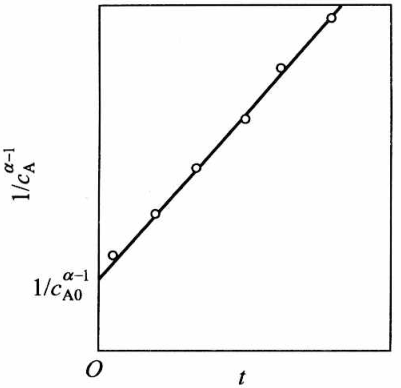
\includegraphics[height=2.7cm]{figs/fig2.6.png}
    \end{columns}        
        以时间$t$对$\frac{1}{c_{\mathrm{A}}^{\alpha-1}}$作图应得一直线，其斜率为$k(\alpha-1)$。但是$k$和$\alpha$均是要求的参数，都是未知值。因此，需先假定$\alpha$的值，根据实验测得的不同时间$t$时组分浓度$c_\mathrm{A}$的数据，按上述方法作图，若得一直线，表明所设$\alpha$值正确，否则需重新假定$\alpha$值，直到获得直线为止。
        \\还须指出，实验必须在等温下进行，这样才能保持$k$为常数。
\end{frame}


\begin{frame}{积分法求反应级数$\alpha$和反应速率常数$k$}
    \begin{table}        
        \caption{简单级数反应特征}
        \begin{tabular}{c l l l l}
            \Xhline{1pt}
            级数 & \makecell[c]{速率方程} & \makecell[c]{速率方程积分式} & \makecell[c]{线性关系} & \makecell[c]{$t$和$c_\mathrm{A}$关系}\\
            \hline
            \rule{0pt}{16pt} 1 & $r=kc_\mathrm{A}$ & $\ln c_\mathrm{A}=-kt+\ln c_\mathrm{A0}$ & $t\sim \ln c_\mathrm{A}$ & $t=\frac{1}{k}\ln\frac{c_\mathrm{A0}}{c_\mathrm{A}}$\\
            \rule{0pt}{16pt} 2 & $r=kc_\mathrm{A}^2$ & $\frac{1}{c_\mathrm{A}}=kt + \frac{1}{c_\mathrm{A0}}$ & $t\sim \frac{1}{c_\mathrm{A}}$ & $t=\frac{1}{k}(\frac{1}{c_\mathrm{A}}-\frac{1}{c_\mathrm{A0}})$ \\
            \rule{0pt}{16pt} 0 & $r=k$ & $c_\mathrm{A}=-kt+c_\mathrm{A0}$ & $t\sim c_\mathrm{A}$ & $t=\frac{1}{k}(c_\mathrm{A0}-c_\mathrm{A})$\\
            \Xhline{1pt}
        \end{tabular}        
\end{table}
\end{frame}


\begin{frame}{积分法求吸附平衡常数$K_\mathrm{A}$和反应速率常数$k$}
    又如速率方程
    $$r_\mathrm{A}=\frac{kK_\mathrm{A}p_\mathrm{A}}{1+K_\mathrm{A}p_\mathrm{A}}$$
    要用积分法求参数$k$和$K_\mathrm{A}$，需先将该式积分，但需首先确定反应速率$r_\mathrm{A}$的表示方式。若为气固相催化反应，常用$-\frac{\mathrm{d}F_\mathrm{A}}{\mathrm{d}W}$来表示，所以
    $$-\frac{\mathrm{d}F_\mathrm{A}}{\mathrm{d}W}=\frac{kK_\mathrm{A}p_\mathrm{A}}{1+K_\mathrm{A}p_\mathrm{A}}$$
    要积分上式，首先要把$F_\mathrm{A}$和$p_\mathrm{A}$变成转化率$X_\mathrm{A}$的函数。对于恒容过程，
    $$F_\mathrm{A}=F_\mathrm{A0}(1-X_\mathrm{A})$$
    $$p_\mathrm{A}=Py_\mathrm{A0}(1-X_\mathrm{A})$$
\end{frame}


\begin{frame}{积分法求吸附平衡常数$K_\mathrm{A}$和反应速率常数$k$}
    $$F_\mathrm{A0}\frac{\mathrm{d}X_\mathrm{A}}{\mathrm{d}W}=\frac{kK_\mathrm{A}Py_\mathrm{A0}(1-X_\mathrm{A})}{1+K_\mathrm{A}Py_\mathrm{A0}(1-X_\mathrm{A})}$$
    积分之，
    $$\int_0^W \frac{\mathrm{d}W}{F_\mathrm{A0}}= \int_0^{X_\mathrm{A}}\frac{1+K_\mathrm{A}Py_\mathrm{A0}(1-X_\mathrm{A})}{kK_\mathrm{A}Py_\mathrm{A0}(1-X_\mathrm{A})}\mathrm{d}X_\mathrm{A}$$
    $$\frac{W}{F_{\mathrm{A} 0}}=\frac{X_{\mathrm{A}}}{k}-\frac{\ln \left(1-X_{\mathrm{A}}\right)}{k K_{\mathrm{A}} P y_{\mathrm{A} 0}} \quad \text{或}\quad  \frac{W}{F_{\mathrm{A} 0} X_{\mathrm{A}}}=\frac{1}{k}-\frac{\ln \left(1-X_{\mathrm{A}}\right)}{k K_{\mathrm{A}} P y_{\mathrm{A} 0} X_{\mathrm{A}}}$$
    当压力、温度、起始气体组成以及催化剂用量一定情况下，改变$F_\mathrm{A0}$进行实验，分别测定相应转化率，根据所得数据，以$\ln(1-X_{\mathrm{A}})/X_{\mathrm{A}}$对$W/F_{\mathrm{A0}}X_{\mathrm{A}}$作图，可得一直线，斜率为$\frac{1}{kK_\mathrm{A}Py_\mathrm{A0}}$，截距为$1/k$,据此算出$k$和$K_{\mathrm{A}}$。    
\end{frame}


\begin{frame}{微分法求反应级数$\alpha$和反应速率常数$k$}
    微分法是根据不同实验条件下测得的反应速率，直接由速率方程估计参数值。仍以$r_\mathrm{A}=kc_\mathrm{A}^\alpha$为例，两边取对数则有
    $$\ln r_\mathrm{A}=\alpha \ln c_\mathrm{A} + \ln k$$
    根据实验数据，作$c_\mathrm{A} \sim t$曲线，在曲线上取若干点作切线求斜率，便得到不同时刻的$-\mathrm{d}c_\mathrm{A}/\mathrm{d}t$，即$r$。再以$\ln c_\mathrm{A}$对$\ln r_\mathrm{A}$作图，应得一直线，直线的斜率等于$\alpha$，截距等于$\ln k$。这样便可将参数值估算出来。
    \\也可以测定不同初始浓度时的初速率$r_0$，再以$\ln c_\mathrm{A}$对$\ln r_0$作图，求反应参数。因为在反应初始阶段，变化比较简单，复杂的因素较少。
\end{frame}


\begin{frame}{微分法求吸附平衡常数$K_\mathrm{A}$和反应速率常数$k$}
    又如速率方程
    $$r_\mathrm{A}=\frac{kK_\mathrm{A}p_\mathrm{A}}{1+K_\mathrm{A}p_\mathrm{A}}$$
    可改写成
    $$\frac{p_{\mathrm{A}}}{r_{\mathrm{A}}}=\frac{1}{k} p_{\mathrm{A}}+\frac{1}{k K_{\mathrm{A}}}$$
    以$\frac{p_{\mathrm{A}}}{r_{\mathrm{A}}}$对$p_{\mathrm{A}}$作图，得一直线，斜率为$1/k$，截距为$1/(kK_\mathrm{A})$。于是动力学参数$k$和$K_\mathrm{A}$可求定。
\end{frame}


\begin{frame}
    \frametitle{}
        \begin{figure}[htpb]
            \centering
            
\includegraphics[width=.9\linewidth]{2.10}
        \end{figure}
\end{frame}


\begin{frame}[t]
    \frametitle{}
    \begin{block}{例2.11}
        由实验测得镍催化剂上苯气相加氢反应的反应速率常数$k$及苯的吸附平衡常数$K_\mathrm{B}$与温度的关系如下表所示：
        \begin{table}
            \centering
            \begin{tabular}{ccccc}
                \bottomrule
                $T$(K) & 363 & 393 & 423 & 453\\ \hline
                $k$[\si{mol/(g.h.MPa^{1.5})}] & 14.52 & 25.96 & 45.07 & 66.03 \\ \hline
                $K_\mathrm{B}$(\si{MPa^{-1}}) & 1495 & 537.3 & 237.9 & 99.41\\  \toprule
            \end{tabular}
        \end{table}
        试求该反应的活化能及苯的吸附热。
        \tcblower
        提示：
        \[
            k = A\exp([-E/RT])
        \]
        \[
            K_\mathrm{B} = K_\mathrm{B0}\exp([q/RT])
        \]
    \end{block}
\end{frame}


\begin{frame}
    \frametitle{}
    \vspace{-0.5em}
    \begin{question}
        在铂催化剂上 ， 乙烯深度氧化的动力学方程可表示为
        \[
            r = \frac{kp_\mathrm{A}p_\mathrm{B}}{(1+K_\mathrm{B}p_\mathrm{B})^2}
        \]
        式中，$p_\mathrm{A}$、 $p_\mathrm{B}$分别为乙烯及氧的分压。在473K 等温下的实验数据如下表。试求该反应温度下的反应速率常数$k$和吸附平衡常数$K_\mathrm{B}$。
        \vspace{-0.5em}
        \begin{table}
            \centering
            \small
            \begin{tabular}{cccc||cccc}
                \bottomrule
                 & \begin{tabular}[c]{@{}c@{}}$p_\mathrm{A}\times 10^3$\\$\mathrm{MPa}$\end{tabular} & \begin{tabular}[c]{@{}c@{}}$p_\mathrm{B}\times 10^3$\\$\mathrm{MPa}$\end{tabular} & \begin{tabular}[c]{@{}c@{}}$r\times 10^4$\\$[\si{mol/(g.min)}]$\end{tabular} &  & \begin{tabular}[c]{@{}c@{}}$p_\mathrm{A}\times 10^3$\\$\mathrm{MPa}$\end{tabular} & \begin{tabular}[c]{@{}c@{}}$p_\mathrm{B}\times 10^3$\\$\mathrm{MPa}$\end{tabular} & \begin{tabular}[c]{@{}c@{}}$r\times 10^4$\\$[\si{mol/(g.min)}]$\end{tabular}\\ \hline
                1 & 8.99 & 3.23 & 0.672 & 7 & 7.75 & 1.82 & 0.828 \\ 
                2 & 14.22 & 3.00 & 1.072 & 8 & 6.17 & 1.73 & 0.656 \\ 
                3 & 8.86 & 4.08 & 0.598 & 9 & 6.13 & 1.73 & 0.694 \\ 
                4 & 8.32 & 2.03 & 0.713 & 10 & 6.98 & 1.56 & 0.791 \\ 
                5 & 4.37 & 0.89 & 0.610 & 11 & 2.87 & 1.06 & 0.418 \\ 
                6 & 7.75 & 1.74 & 0.834 &  &  &  &  \\ \toprule
            \end{tabular}
        \end{table}
        \vspace{-1.5em}
    \end{question}
\end{frame}




\end{document}